% Options for packages loaded elsewhere
\PassOptionsToPackage{unicode}{hyperref}
\PassOptionsToPackage{hyphens}{url}
\PassOptionsToPackage{dvipsnames,svgnames,x11names}{xcolor}
%
\documentclass[
  letterpaper,
  DIV=11,
  numbers=noendperiod]{scrartcl}

\usepackage{amsmath,amssymb}
\usepackage{iftex}
\ifPDFTeX
  \usepackage[T1]{fontenc}
  \usepackage[utf8]{inputenc}
  \usepackage{textcomp} % provide euro and other symbols
\else % if luatex or xetex
  \usepackage{unicode-math}
  \defaultfontfeatures{Scale=MatchLowercase}
  \defaultfontfeatures[\rmfamily]{Ligatures=TeX,Scale=1}
\fi
\usepackage{lmodern}
\ifPDFTeX\else  
    % xetex/luatex font selection
\fi
% Use upquote if available, for straight quotes in verbatim environments
\IfFileExists{upquote.sty}{\usepackage{upquote}}{}
\IfFileExists{microtype.sty}{% use microtype if available
  \usepackage[]{microtype}
  \UseMicrotypeSet[protrusion]{basicmath} % disable protrusion for tt fonts
}{}
\makeatletter
\@ifundefined{KOMAClassName}{% if non-KOMA class
  \IfFileExists{parskip.sty}{%
    \usepackage{parskip}
  }{% else
    \setlength{\parindent}{0pt}
    \setlength{\parskip}{6pt plus 2pt minus 1pt}}
}{% if KOMA class
  \KOMAoptions{parskip=half}}
\makeatother
\usepackage{xcolor}
\setlength{\emergencystretch}{3em} % prevent overfull lines
\setcounter{secnumdepth}{-\maxdimen} % remove section numbering
% Make \paragraph and \subparagraph free-standing
\ifx\paragraph\undefined\else
  \let\oldparagraph\paragraph
  \renewcommand{\paragraph}[1]{\oldparagraph{#1}\mbox{}}
\fi
\ifx\subparagraph\undefined\else
  \let\oldsubparagraph\subparagraph
  \renewcommand{\subparagraph}[1]{\oldsubparagraph{#1}\mbox{}}
\fi

\usepackage{color}
\usepackage{fancyvrb}
\newcommand{\VerbBar}{|}
\newcommand{\VERB}{\Verb[commandchars=\\\{\}]}
\DefineVerbatimEnvironment{Highlighting}{Verbatim}{commandchars=\\\{\}}
% Add ',fontsize=\small' for more characters per line
\newenvironment{Shaded}{}{}
\newcommand{\AlertTok}[1]{\textcolor[rgb]{1.00,0.33,0.33}{\textbf{#1}}}
\newcommand{\AnnotationTok}[1]{\textcolor[rgb]{0.42,0.45,0.49}{#1}}
\newcommand{\AttributeTok}[1]{\textcolor[rgb]{0.84,0.23,0.29}{#1}}
\newcommand{\BaseNTok}[1]{\textcolor[rgb]{0.00,0.36,0.77}{#1}}
\newcommand{\BuiltInTok}[1]{\textcolor[rgb]{0.84,0.23,0.29}{#1}}
\newcommand{\CharTok}[1]{\textcolor[rgb]{0.01,0.18,0.38}{#1}}
\newcommand{\CommentTok}[1]{\textcolor[rgb]{0.42,0.45,0.49}{#1}}
\newcommand{\CommentVarTok}[1]{\textcolor[rgb]{0.42,0.45,0.49}{#1}}
\newcommand{\ConstantTok}[1]{\textcolor[rgb]{0.00,0.36,0.77}{#1}}
\newcommand{\ControlFlowTok}[1]{\textcolor[rgb]{0.84,0.23,0.29}{#1}}
\newcommand{\DataTypeTok}[1]{\textcolor[rgb]{0.84,0.23,0.29}{#1}}
\newcommand{\DecValTok}[1]{\textcolor[rgb]{0.00,0.36,0.77}{#1}}
\newcommand{\DocumentationTok}[1]{\textcolor[rgb]{0.42,0.45,0.49}{#1}}
\newcommand{\ErrorTok}[1]{\textcolor[rgb]{1.00,0.33,0.33}{\underline{#1}}}
\newcommand{\ExtensionTok}[1]{\textcolor[rgb]{0.84,0.23,0.29}{\textbf{#1}}}
\newcommand{\FloatTok}[1]{\textcolor[rgb]{0.00,0.36,0.77}{#1}}
\newcommand{\FunctionTok}[1]{\textcolor[rgb]{0.44,0.26,0.76}{#1}}
\newcommand{\ImportTok}[1]{\textcolor[rgb]{0.01,0.18,0.38}{#1}}
\newcommand{\InformationTok}[1]{\textcolor[rgb]{0.42,0.45,0.49}{#1}}
\newcommand{\KeywordTok}[1]{\textcolor[rgb]{0.84,0.23,0.29}{#1}}
\newcommand{\NormalTok}[1]{\textcolor[rgb]{0.14,0.16,0.18}{#1}}
\newcommand{\OperatorTok}[1]{\textcolor[rgb]{0.14,0.16,0.18}{#1}}
\newcommand{\OtherTok}[1]{\textcolor[rgb]{0.44,0.26,0.76}{#1}}
\newcommand{\PreprocessorTok}[1]{\textcolor[rgb]{0.84,0.23,0.29}{#1}}
\newcommand{\RegionMarkerTok}[1]{\textcolor[rgb]{0.42,0.45,0.49}{#1}}
\newcommand{\SpecialCharTok}[1]{\textcolor[rgb]{0.00,0.36,0.77}{#1}}
\newcommand{\SpecialStringTok}[1]{\textcolor[rgb]{0.01,0.18,0.38}{#1}}
\newcommand{\StringTok}[1]{\textcolor[rgb]{0.01,0.18,0.38}{#1}}
\newcommand{\VariableTok}[1]{\textcolor[rgb]{0.89,0.38,0.04}{#1}}
\newcommand{\VerbatimStringTok}[1]{\textcolor[rgb]{0.01,0.18,0.38}{#1}}
\newcommand{\WarningTok}[1]{\textcolor[rgb]{1.00,0.33,0.33}{#1}}

\providecommand{\tightlist}{%
  \setlength{\itemsep}{0pt}\setlength{\parskip}{0pt}}\usepackage{longtable,booktabs,array}
\usepackage{calc} % for calculating minipage widths
% Correct order of tables after \paragraph or \subparagraph
\usepackage{etoolbox}
\makeatletter
\patchcmd\longtable{\par}{\if@noskipsec\mbox{}\fi\par}{}{}
\makeatother
% Allow footnotes in longtable head/foot
\IfFileExists{footnotehyper.sty}{\usepackage{footnotehyper}}{\usepackage{footnote}}
\makesavenoteenv{longtable}
\usepackage{graphicx}
\makeatletter
\def\maxwidth{\ifdim\Gin@nat@width>\linewidth\linewidth\else\Gin@nat@width\fi}
\def\maxheight{\ifdim\Gin@nat@height>\textheight\textheight\else\Gin@nat@height\fi}
\makeatother
% Scale images if necessary, so that they will not overflow the page
% margins by default, and it is still possible to overwrite the defaults
% using explicit options in \includegraphics[width, height, ...]{}
\setkeys{Gin}{width=\maxwidth,height=\maxheight,keepaspectratio}
% Set default figure placement to htbp
\makeatletter
\def\fps@figure{htbp}
\makeatother

\KOMAoption{captions}{tableheading}
\makeatletter
\makeatother
\makeatletter
\makeatother
\makeatletter
\@ifpackageloaded{caption}{}{\usepackage{caption}}
\AtBeginDocument{%
\ifdefined\contentsname
  \renewcommand*\contentsname{Table of contents}
\else
  \newcommand\contentsname{Table of contents}
\fi
\ifdefined\listfigurename
  \renewcommand*\listfigurename{List of Figures}
\else
  \newcommand\listfigurename{List of Figures}
\fi
\ifdefined\listtablename
  \renewcommand*\listtablename{List of Tables}
\else
  \newcommand\listtablename{List of Tables}
\fi
\ifdefined\figurename
  \renewcommand*\figurename{Figure}
\else
  \newcommand\figurename{Figure}
\fi
\ifdefined\tablename
  \renewcommand*\tablename{Table}
\else
  \newcommand\tablename{Table}
\fi
}
\@ifpackageloaded{float}{}{\usepackage{float}}
\floatstyle{ruled}
\@ifundefined{c@chapter}{\newfloat{codelisting}{h}{lop}}{\newfloat{codelisting}{h}{lop}[chapter]}
\floatname{codelisting}{Listing}
\newcommand*\listoflistings{\listof{codelisting}{List of Listings}}
\makeatother
\makeatletter
\@ifpackageloaded{caption}{}{\usepackage{caption}}
\@ifpackageloaded{subcaption}{}{\usepackage{subcaption}}
\makeatother
\makeatletter
\@ifpackageloaded{tcolorbox}{}{\usepackage[skins,breakable]{tcolorbox}}
\makeatother
\makeatletter
\@ifundefined{shadecolor}{\definecolor{shadecolor}{rgb}{.97, .97, .97}}
\makeatother
\makeatletter
\makeatother
\makeatletter
\makeatother
\ifLuaTeX
  \usepackage{selnolig}  % disable illegal ligatures
\fi
\IfFileExists{bookmark.sty}{\usepackage{bookmark}}{\usepackage{hyperref}}
\IfFileExists{xurl.sty}{\usepackage{xurl}}{} % add URL line breaks if available
\urlstyle{same} % disable monospaced font for URLs
\hypersetup{
  pdftitle={Travail pratique VID},
  pdfauthor={Julien Muhlemann},
  colorlinks=true,
  linkcolor={blue},
  filecolor={Maroon},
  citecolor={Blue},
  urlcolor={Blue},
  pdfcreator={LaTeX via pandoc}}

\title{Travail pratique VID}
\usepackage{etoolbox}
\makeatletter
\providecommand{\subtitle}[1]{% add subtitle to \maketitle
  \apptocmd{\@title}{\par {\large #1 \par}}{}{}
}
\makeatother
\subtitle{TP \#1}
\author{Julien Muhlemann}
\date{26 March, 2024}

\begin{document}
\maketitle
\ifdefined\Shaded\renewenvironment{Shaded}{\begin{tcolorbox}[enhanced, borderline west={3pt}{0pt}{shadecolor}, interior hidden, breakable, boxrule=0pt, frame hidden, sharp corners]}{\end{tcolorbox}}\fi

\renewcommand*\contentsname{Table of contents}
{
\hypersetup{linkcolor=}
\setcounter{tocdepth}{3}
\tableofcontents
}
Introduction

Dans ce travail pratique, nous allons explorer l'utilisation du logiciel
R pour l'analyse de données. À travers cet exercice, nous renforcerons
nos compétences en analyse exploratoire et en visualisation de données,
tout en apprenant à rédiger des rapports d'analyse clairs et concis.

Guidés par des ressources pédagogiques disponibles, nous aurons
l'opportunité de manipuler différents jeux de données et d'acquérir une
meilleure compréhension des techniques statistiques utilisées en science
des données.

\begin{Shaded}
\begin{Highlighting}[]
\FunctionTok{library}\NormalTok{(readxl)}
\FunctionTok{library}\NormalTok{(e1071)}
\end{Highlighting}
\end{Shaded}

Q1A:

Voici le code permettant de charger les donnée des notes:\\

\begin{Shaded}
\begin{Highlighting}[]
\NormalTok{examen }\OtherTok{\textless{}{-}} \FunctionTok{read\_xlsx}\NormalTok{(}\StringTok{"Notes.xlsx"}\NormalTok{)}
\end{Highlighting}
\end{Shaded}

Q1B:

Voici le code permettant d'afficher les boxplots:

\begin{Shaded}
\begin{Highlighting}[]
\FunctionTok{par}\NormalTok{(}\AttributeTok{mfrow=}\FunctionTok{c}\NormalTok{(}\DecValTok{1}\NormalTok{,}\DecValTok{2}\NormalTok{), }\AttributeTok{pty=}\StringTok{"s"}\NormalTok{)}

\FunctionTok{boxplot}\NormalTok{(Note }\SpecialCharTok{\textasciitilde{}}\NormalTok{ Classe, }\AttributeTok{data =}\NormalTok{ examen, }\AttributeTok{main =} \StringTok{"Notes de l\textquotesingle{}examen de mathématiques"}\NormalTok{, }\AttributeTok{xlab =} \StringTok{"Classe"}\NormalTok{, }\AttributeTok{ylab =} \StringTok{"Note"}\NormalTok{, }\AttributeTok{col =} \StringTok{"orange"}\NormalTok{)}

\FunctionTok{abline}\NormalTok{(}\AttributeTok{h =} \DecValTok{4}\NormalTok{, }\AttributeTok{col =} \StringTok{"black"}\NormalTok{, }\AttributeTok{lty =} \DecValTok{2}\NormalTok{)}
\end{Highlighting}
\end{Shaded}

\begin{figure}[H]

{\centering 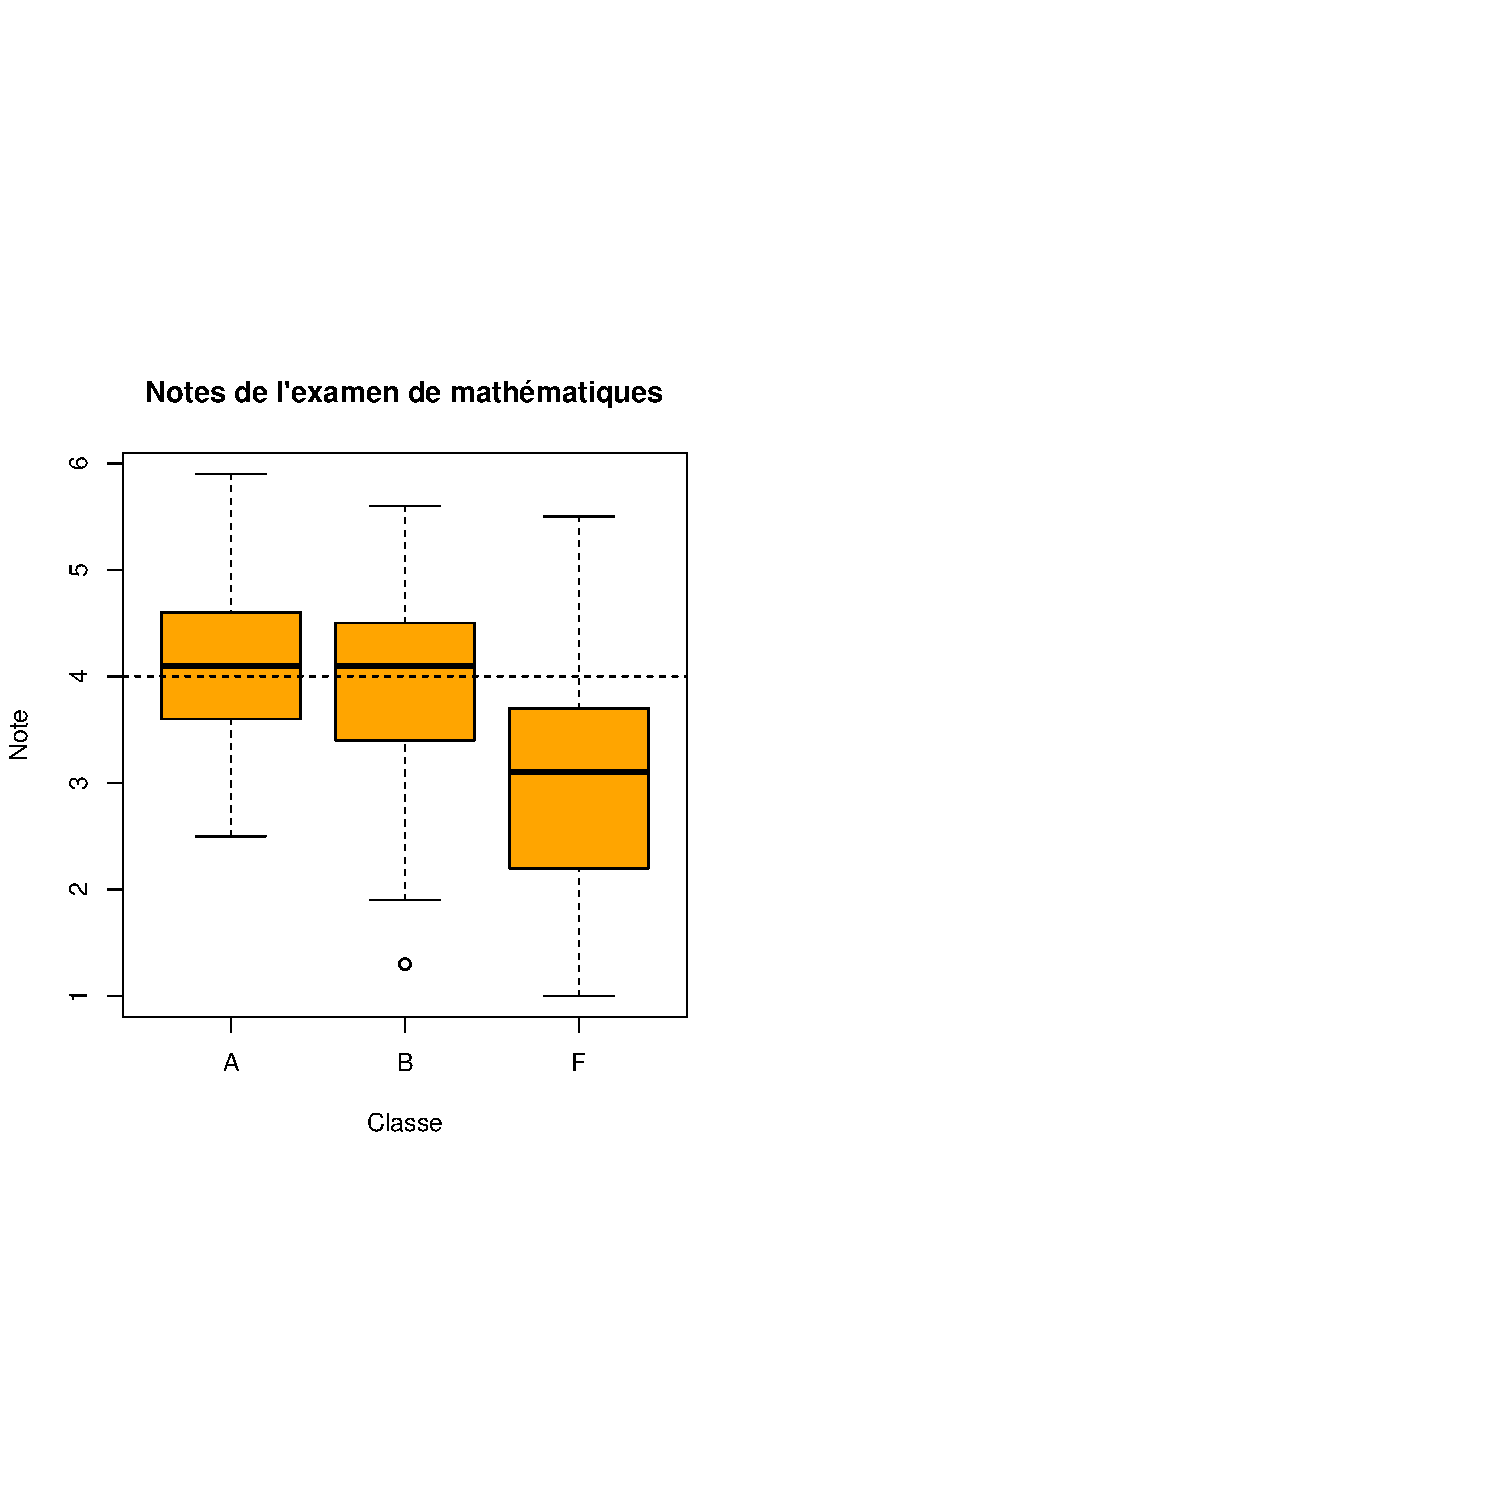
\includegraphics{pw1_VID_files/figure-pdf/unnamed-chunk-3-1.pdf}

}

\end{figure}

Q1C:

Il existe en effet une différence significative entre la classe `F' et
la classe `A'. L'intervalle de travail de la classe `F' est beaucoup
plus grand {[}1 ; 5.5{]} alors que la classe `A' {[}2.5 ; 6{]} réussi un
peu mieux son examen de mathématique. En conséquence la moyenne (donc la
position) est plus élevée dans la classe `A'. Quant à la classe `B' elle
se trouve entre les deux autres avec une moyenne très proche de la
classe `A'.

Q1D:

Oui en effet, nous pouvons utiliser un indicateur de dispersion tel que
l'écart-type ou l'IQR avec la fonction IQR(). Nous pouvons voir que
l'IQR est plus élevé pour la classe `F'. Attention il convient de garder
en tête que nous avons ôté les valeur NA donc les jeux de données sont
potentiellement non équilibrés.

\begin{Shaded}
\begin{Highlighting}[]
\FunctionTok{print}\NormalTok{(}\FunctionTok{IQR}\NormalTok{(examen}\SpecialCharTok{$}\NormalTok{Note[examen}\SpecialCharTok{$}\NormalTok{Classe }\SpecialCharTok{==} \StringTok{\textquotesingle{}A\textquotesingle{}}\NormalTok{], }\AttributeTok{na.rm =}\ConstantTok{TRUE}\NormalTok{))}
\end{Highlighting}
\end{Shaded}

\begin{verbatim}
[1] 1
\end{verbatim}

\begin{Shaded}
\begin{Highlighting}[]
\FunctionTok{print}\NormalTok{(}\FunctionTok{IQR}\NormalTok{(examen}\SpecialCharTok{$}\NormalTok{Note[examen}\SpecialCharTok{$}\NormalTok{Classe }\SpecialCharTok{==} \StringTok{\textquotesingle{}B\textquotesingle{}}\NormalTok{], }\AttributeTok{na.rm =}\ConstantTok{TRUE}\NormalTok{))}
\end{Highlighting}
\end{Shaded}

\begin{verbatim}
[1] 1.05
\end{verbatim}

\begin{Shaded}
\begin{Highlighting}[]
\FunctionTok{print}\NormalTok{(}\FunctionTok{IQR}\NormalTok{(examen}\SpecialCharTok{$}\NormalTok{Note[examen}\SpecialCharTok{$}\NormalTok{Classe }\SpecialCharTok{==} \StringTok{\textquotesingle{}F\textquotesingle{}}\NormalTok{], }\AttributeTok{na.rm =}\ConstantTok{TRUE}\NormalTok{))}
\end{Highlighting}
\end{Shaded}

\begin{verbatim}
[1] 1.5
\end{verbatim}

Q1E:

Les calculs des écarts-types selon le fonction sd et by. Oui il existe
une différence entre les classes `F' et les deux autres classes `A' et
`B' comme décrit plus haut.

\begin{Shaded}
\begin{Highlighting}[]
\FunctionTok{print}\NormalTok{(}\FunctionTok{paste}\NormalTok{(}\StringTok{"STD A:"}\NormalTok{, }\FunctionTok{sd}\NormalTok{(examen}\SpecialCharTok{$}\NormalTok{Note[examen}\SpecialCharTok{$}\NormalTok{Classe }\SpecialCharTok{==} \StringTok{\textquotesingle{}A\textquotesingle{}}\NormalTok{], }\AttributeTok{na.rm =}\ConstantTok{TRUE}\NormalTok{)))}
\end{Highlighting}
\end{Shaded}

\begin{verbatim}
[1] "STD A: 0.848528137423857"
\end{verbatim}

\begin{Shaded}
\begin{Highlighting}[]
\FunctionTok{print}\NormalTok{(}\FunctionTok{paste}\NormalTok{(}\StringTok{"STD B:"}\NormalTok{, }\FunctionTok{sd}\NormalTok{(examen}\SpecialCharTok{$}\NormalTok{Note[examen}\SpecialCharTok{$}\NormalTok{Classe }\SpecialCharTok{==} \StringTok{\textquotesingle{}B\textquotesingle{}}\NormalTok{], }\AttributeTok{na.rm =}\ConstantTok{TRUE}\NormalTok{)))}
\end{Highlighting}
\end{Shaded}

\begin{verbatim}
[1] "STD B: 1.00166528008778"
\end{verbatim}

\begin{Shaded}
\begin{Highlighting}[]
\FunctionTok{print}\NormalTok{(}\FunctionTok{paste}\NormalTok{(}\StringTok{"STD F:"}\NormalTok{, }\FunctionTok{sd}\NormalTok{(examen}\SpecialCharTok{$}\NormalTok{Note[examen}\SpecialCharTok{$}\NormalTok{Classe }\SpecialCharTok{==} \StringTok{\textquotesingle{}F\textquotesingle{}}\NormalTok{], }\AttributeTok{na.rm =}\ConstantTok{TRUE}\NormalTok{)))}
\end{Highlighting}
\end{Shaded}

\begin{verbatim}
[1] "STD F: 1.30986004341431"
\end{verbatim}

\begin{Shaded}
\begin{Highlighting}[]
\FunctionTok{print}\NormalTok{(}\FunctionTok{paste}\NormalTok{(}\StringTok{"STD A:"}\NormalTok{, }\FunctionTok{by}\NormalTok{(examen}\SpecialCharTok{$}\NormalTok{Note, examen}\SpecialCharTok{$}\NormalTok{Classe }\SpecialCharTok{==} \StringTok{\textquotesingle{}A\textquotesingle{}}\NormalTok{, sd, }\AttributeTok{na.rm =}\NormalTok{ T)))}
\end{Highlighting}
\end{Shaded}

\begin{verbatim}
[1] "STD A: 1.21701769727137"  "STD A: 0.848528137423857"
\end{verbatim}

\begin{Shaded}
\begin{Highlighting}[]
\FunctionTok{print}\NormalTok{(}\FunctionTok{paste}\NormalTok{(}\StringTok{"STD B:"}\NormalTok{, }\FunctionTok{by}\NormalTok{(examen}\SpecialCharTok{$}\NormalTok{Note, examen}\SpecialCharTok{$}\NormalTok{Classe }\SpecialCharTok{==} \StringTok{\textquotesingle{}B\textquotesingle{}}\NormalTok{, sd, }\AttributeTok{na.rm =}\NormalTok{ T)))}
\end{Highlighting}
\end{Shaded}

\begin{verbatim}
[1] "STD B: 1.21287144531362" "STD B: 1.00166528008778"
\end{verbatim}

\begin{Shaded}
\begin{Highlighting}[]
\FunctionTok{print}\NormalTok{(}\FunctionTok{paste}\NormalTok{(}\StringTok{"STD F:"}\NormalTok{, }\FunctionTok{by}\NormalTok{(examen}\SpecialCharTok{$}\NormalTok{Note, examen}\SpecialCharTok{$}\NormalTok{Classe }\SpecialCharTok{==} \StringTok{\textquotesingle{}F\textquotesingle{}}\NormalTok{, sd, }\AttributeTok{na.rm =}\NormalTok{ T)))}
\end{Highlighting}
\end{Shaded}

\begin{verbatim}
[1] "STD F: 0.930970123098264" "STD F: 1.30986004341431" 
\end{verbatim}

Q1F.

L'écart-type est un indicateur robuste de la dispersion des valeurs d'un
dataset. Il convient comme déjà, dit de tenir compte du nombre
d'observations entre les différentes classes.

Q1G:

Nous commençons par sélectionner la feature `Note' de la classe `A'.
Ensuite nous appelons la fonction summary().

\begin{Shaded}
\begin{Highlighting}[]
\NormalTok{distA }\OtherTok{\textless{}{-}}\NormalTok{ examen}\SpecialCharTok{$}\NormalTok{Note[examen}\SpecialCharTok{$}\NormalTok{Classe }\SpecialCharTok{==} \StringTok{\textquotesingle{}A\textquotesingle{}}\NormalTok{]}
\FunctionTok{summary}\NormalTok{(distA)}
\end{Highlighting}
\end{Shaded}

\begin{verbatim}
   Min. 1st Qu.  Median    Mean 3rd Qu.    Max.    NA's 
   2.50    3.60    4.10    4.08    4.60    5.90       3 
\end{verbatim}

Q1H:

Nous utilisons la fonction skewness. Elle nous informe

1. de la magnitude de l'asymétrie et

2. du sens de celle-ci

Nous obtenons un -0.588 ce qui nous donne une asymétrie négative de
magnitude moyenne. L'histogramme nous le confirme.

\begin{Shaded}
\begin{Highlighting}[]
\FunctionTok{library}\NormalTok{(e1071)}
\NormalTok{distB }\OtherTok{\textless{}{-}}\NormalTok{ examen}\SpecialCharTok{$}\NormalTok{Note[examen}\SpecialCharTok{$}\NormalTok{Classe }\SpecialCharTok{==} \StringTok{\textquotesingle{}B\textquotesingle{}}\NormalTok{]}
\NormalTok{distB }\OtherTok{\textless{}{-}} \FunctionTok{na.omit}\NormalTok{(distB)}

\FunctionTok{print}\NormalTok{(}\FunctionTok{skewness}\NormalTok{(distB))}
\end{Highlighting}
\end{Shaded}

\begin{verbatim}
[1] -0.5881639
\end{verbatim}

\begin{Shaded}
\begin{Highlighting}[]
\FunctionTok{print}\NormalTok{(}\FunctionTok{hist}\NormalTok{(distB))}
\end{Highlighting}
\end{Shaded}

\begin{figure}[H]

{\centering 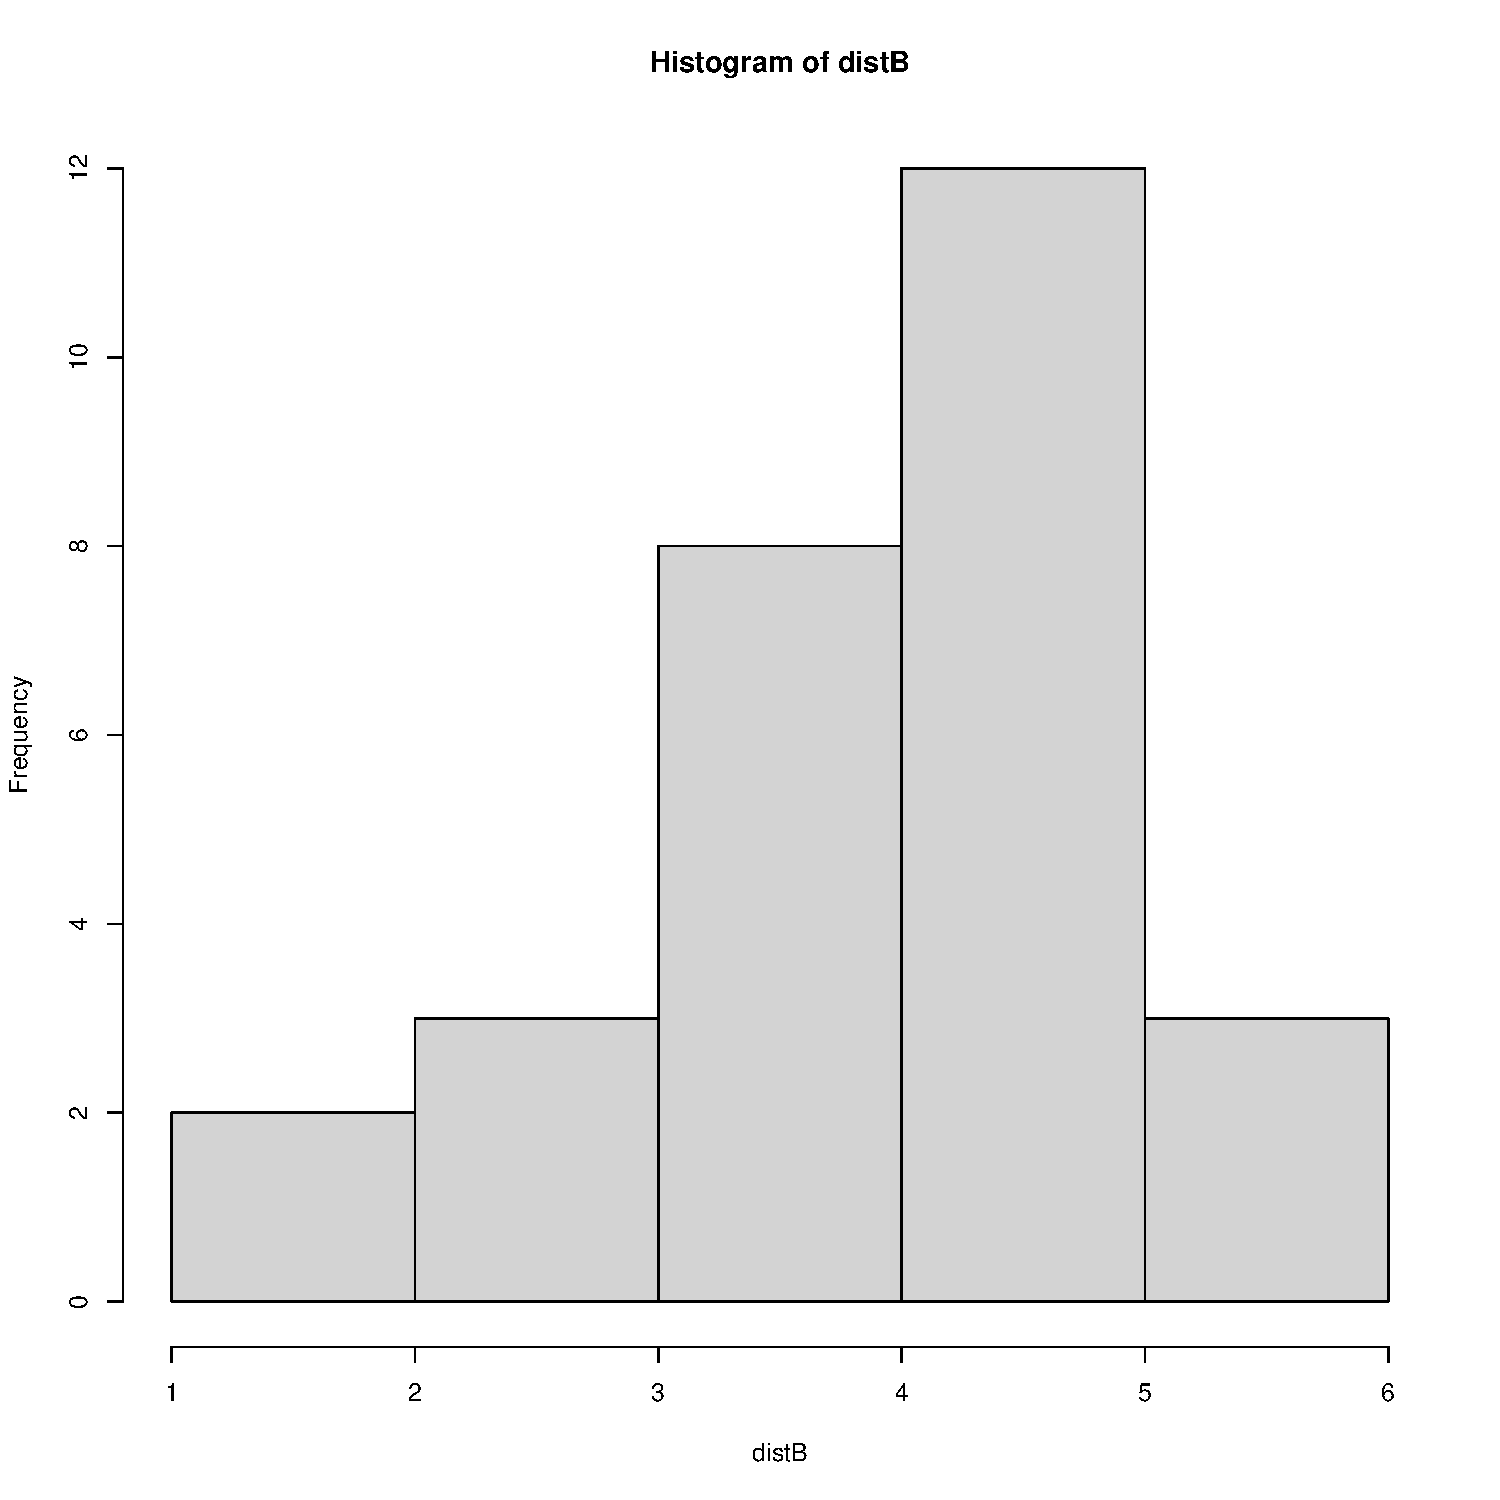
\includegraphics{pw1_VID_files/figure-pdf/unnamed-chunk-8-1.pdf}

}

\end{figure}

\begin{verbatim}
$breaks
[1] 1 2 3 4 5 6

$counts
[1]  2  3  8 12  3

$density
[1] 0.07142857 0.10714286 0.28571429 0.42857143 0.10714286

$mids
[1] 1.5 2.5 3.5 4.5 5.5

$xname
[1] "distB"

$equidist
[1] TRUE

attr(,"class")
[1] "histogram"
\end{verbatim}

Q1I: Les boîtes à moustaches mettent en valeur la dispersion des données
IQR. Quant au diagramme de densité, il montre de manière plus claire le
type de distribution et le mode. Le deux diagrammes sont intéressants
lors de l'analyse. Néanmoins le diagramme en densité semble plus
approprié pour l'exemple des notes.

Q2A:

\begin{Shaded}
\begin{Highlighting}[]
\FunctionTok{library}\NormalTok{(lattice)}
\FunctionTok{data}\NormalTok{(Titanic)}
\FunctionTok{summary}\NormalTok{(Titanic)}
\end{Highlighting}
\end{Shaded}

\begin{verbatim}
Number of cases in table: 2201 
Number of factors: 4 
Test for independence of all factors:
    Chisq = 1637.4, df = 25, p-value = 0
    Chi-squared approximation may be incorrect
\end{verbatim}

Q2B:

Voici le code permettant d'afficher le graphique selon l'exemple: Nous
avons donc dans la `formule' les variable Class et Freq qui doivent être
utilisées. Ensuite les variables conditionnelles Sex et Age qui vont
permettre d'ajouter des en-têtes.

Si l'argument Stack est = True alors nous obtenons plus qu'un seul
histogramme par classe et boîte. Avec ce paramètre la comparaison n'est
plus aussi aisée. Il peut être utilisé dans un cas ou la différence
entre les valeurs à comparer n'est pas significative.

\begin{Shaded}
\begin{Highlighting}[]
\NormalTok{titanic.bar }\OtherTok{\textless{}{-}} \FunctionTok{barchart}\NormalTok{(Class}\SpecialCharTok{\textasciitilde{}}\NormalTok{Freq }\SpecialCharTok{|}\NormalTok{ Sex }\SpecialCharTok{*}\NormalTok{ Age, }\AttributeTok{data=}\FunctionTok{as.data.frame}\NormalTok{(Titanic), }
                      \AttributeTok{groups=}\NormalTok{Survived, }\AttributeTok{stack=}\NormalTok{F, }\AttributeTok{layout=}\FunctionTok{c}\NormalTok{(}\DecValTok{4}\NormalTok{,}\DecValTok{1}\NormalTok{), }
                      \AttributeTok{auto.key=}\FunctionTok{list}\NormalTok{(}\AttributeTok{title=}\StringTok{"Survived"}\NormalTok{, }\AttributeTok{columns=}\DecValTok{2}\NormalTok{))}
\FunctionTok{print}\NormalTok{(titanic.bar)}
\end{Highlighting}
\end{Shaded}

\begin{figure}[H]

{\centering 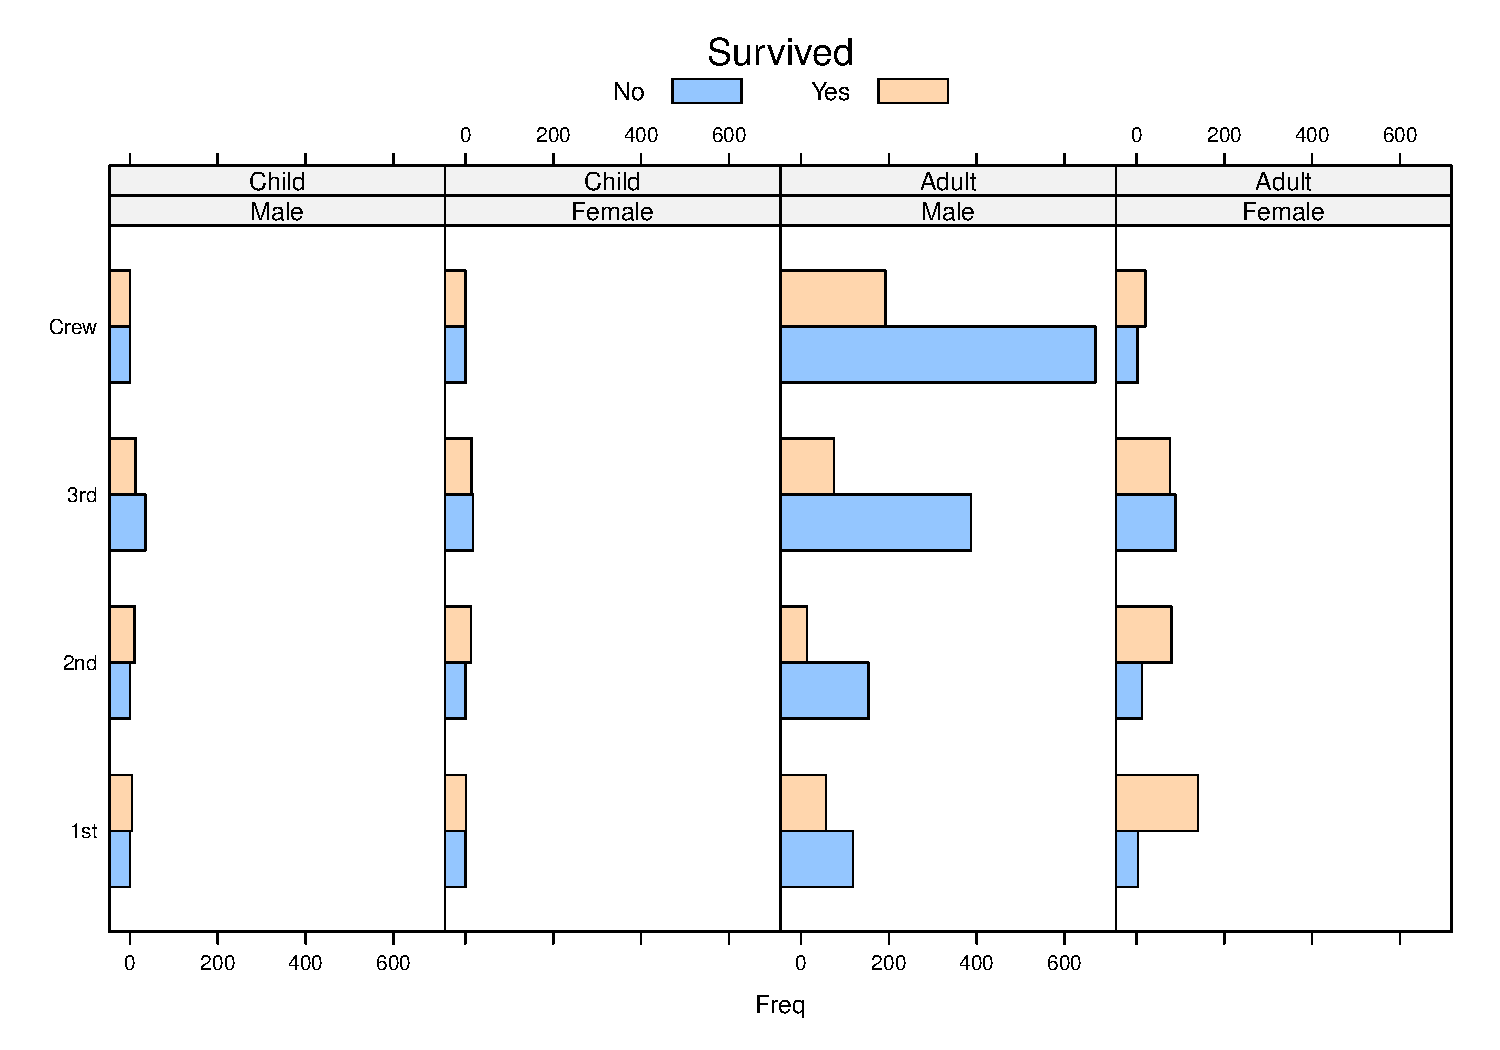
\includegraphics{pw1_VID_files/figure-pdf/unnamed-chunk-10-1.pdf}

}

\end{figure}

Q2C: 1. Oui il existe une différence significative entre les genre dans
la catégorie Adulte. En effet les enfants ne présentent pas de
différence notable entre les survivants vs décédés fille et garçons.

\begin{enumerate}
\def\labelenumi{\arabic{enumi}.}
\setcounter{enumi}{1}
\item
  Oui il y a une différence significative entre les adultes et les
  enfants. En premier lieu il est à noter qu'il y avait plus d'individus
  adultes que enfants à bord. Ensuite, il y a eu beaucoup plus de décès
  chez les adultes que chez les enfants.
\item
  Oui il y a eu (chez les adultes) proportionnellement à la
  représentation de l'échantillon de la classe, plus de décès chez chez
  l'équipage. Ensuite nous observons une diminution du nombre de morts
  en avançant vers les classes plus aisées.
\item
  Interprétation: Les 3ème classes se situaient en fond de bâtiment et
  les cloisons ont été fermées afin de confiner la montée des eaux. En
  outre, leur probabilités de survie ont été diminuées.

  Source:
  https://abc13.com/titanic-anniversary-immigration-world-history/1874040/\#:\textasciitilde:text=Approximately\%201\%2C317\%20passengers\%20died\%20when,their\%20area\%20of\%20the\%20Titanic.
\end{enumerate}

Q2D: On pourrait envisager la présentation d'un histogramme par
combinaison de genre et de sexe (4) avec deux bar-graphes par classes
afin de comparer les survivants comme montré dans le graphe précédent.

Q3A:

\begin{Shaded}
\begin{Highlighting}[]
\FunctionTok{library}\NormalTok{(HSAUR2)}
\FunctionTok{library}\NormalTok{(tools)}

\FunctionTok{par}\NormalTok{(}\AttributeTok{pty=}\StringTok{"s"}\NormalTok{)}
\FunctionTok{plot}\NormalTok{(plasma}\SpecialCharTok{$}\NormalTok{fibrinogen, plasma}\SpecialCharTok{$}\NormalTok{globulin,}
     \AttributeTok{pch =} \DecValTok{20}\NormalTok{, }\AttributeTok{main =} \StringTok{"Nuage de points : Globuline vs.Fibrinogène"}\NormalTok{,}
     \AttributeTok{xlab =} \StringTok{"Globuline"}\NormalTok{,}
     \AttributeTok{ylab =} \StringTok{"Fibrinogène"}\NormalTok{,}
     \AttributeTok{aspect.ratio =} \DecValTok{1}\NormalTok{)}
\end{Highlighting}
\end{Shaded}

\begin{figure}[H]

{\centering 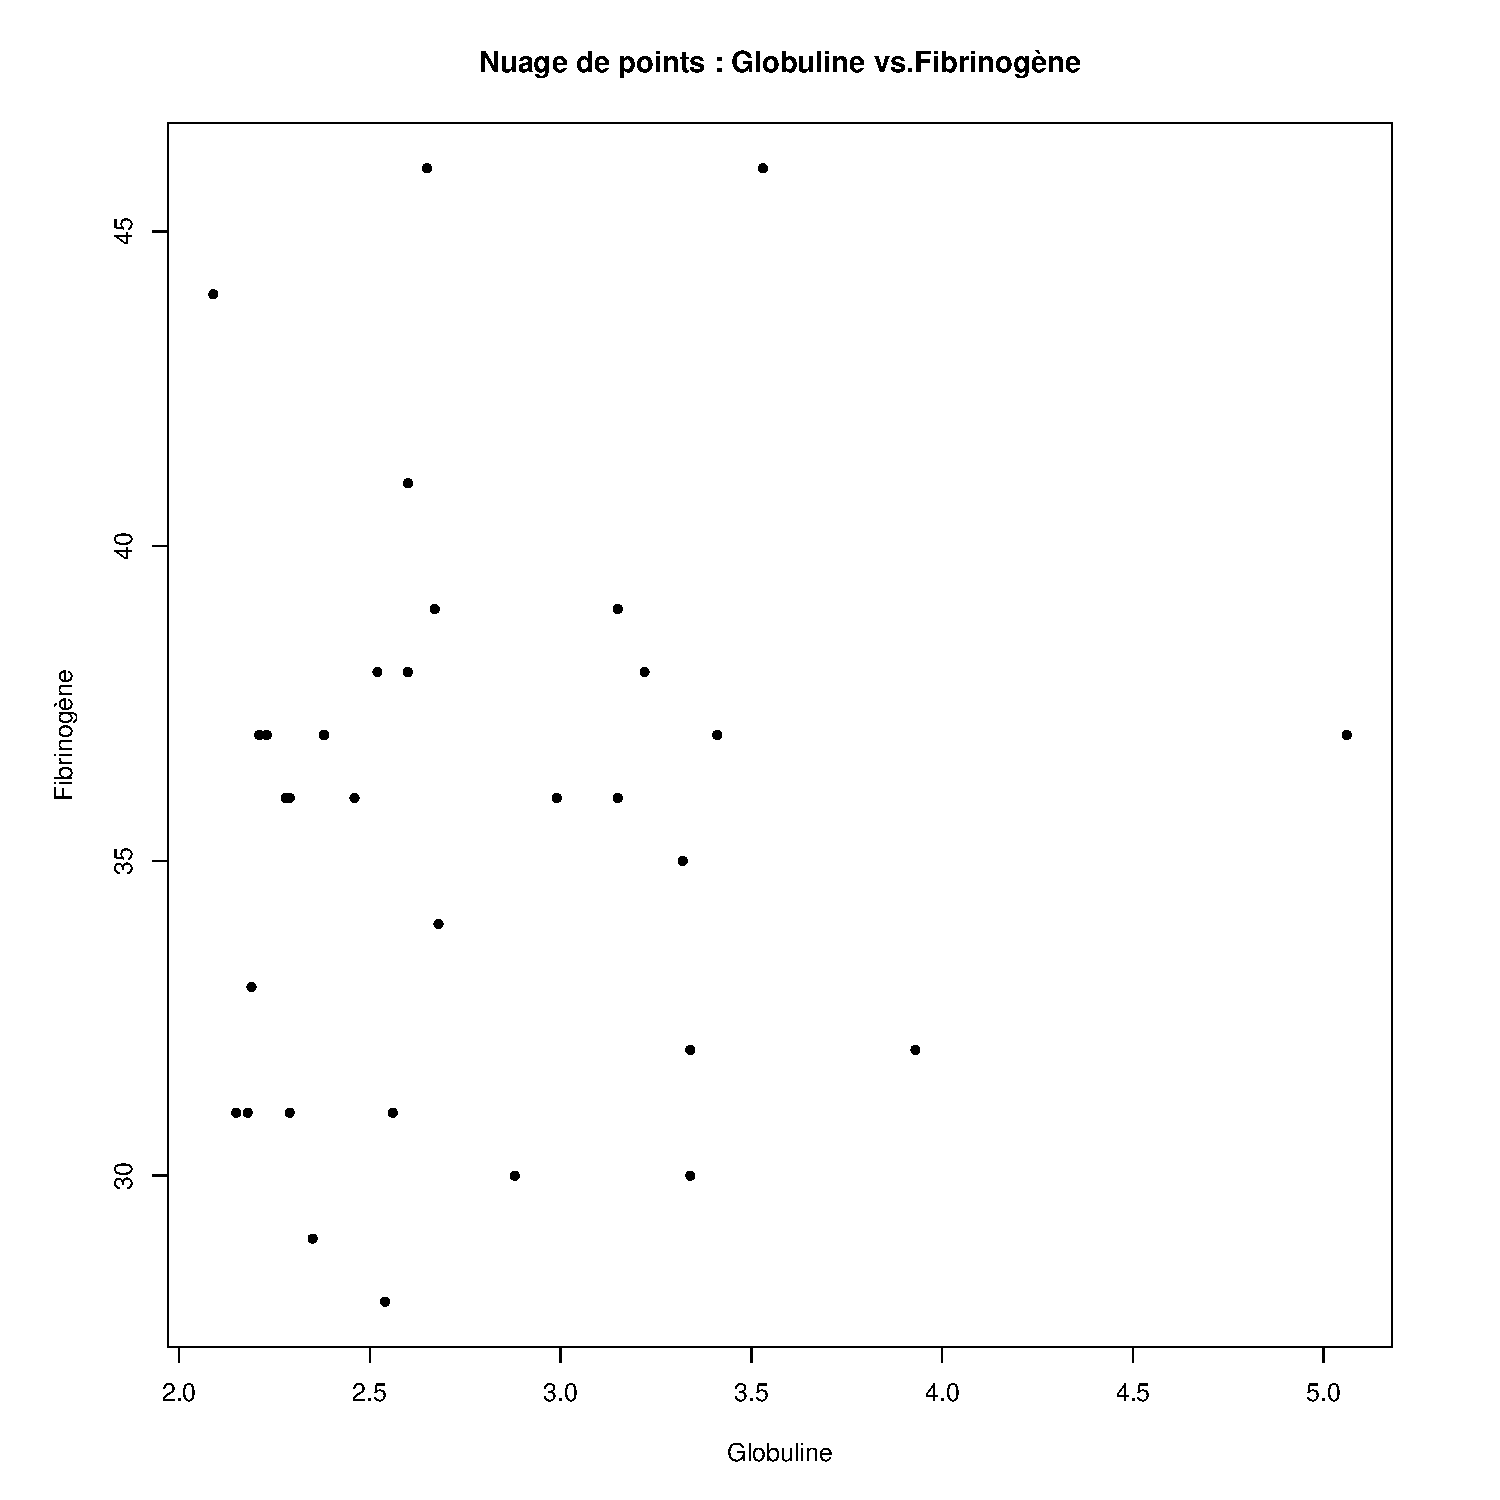
\includegraphics{pw1_VID_files/figure-pdf/unnamed-chunk-11-1.pdf}

}

\end{figure}

Q3B:

Nous pouvons connaître la corrélation avec le code suivant: Nous
obtenons 0.08 nous avons donc aucune linéarité entre les deux variables.

\begin{Shaded}
\begin{Highlighting}[]
\NormalTok{correlation }\OtherTok{\textless{}{-}} \FunctionTok{cor}\NormalTok{(plasma}\SpecialCharTok{$}\NormalTok{fibrinogen, plasma}\SpecialCharTok{$}\NormalTok{globulin)}

\FunctionTok{print}\NormalTok{(correlation)}
\end{Highlighting}
\end{Shaded}

\begin{verbatim}
[1] 0.08071681
\end{verbatim}

Q3C:

\begin{Shaded}
\begin{Highlighting}[]
\NormalTok{plasma.glm}\OtherTok{\textless{}{-}}\FunctionTok{glm}\NormalTok{(ESR}\SpecialCharTok{\textasciitilde{}}\NormalTok{fibrinogen}\SpecialCharTok{+}\NormalTok{globulin, }\AttributeTok{data=}\NormalTok{plasma, }\AttributeTok{family=}\NormalTok{binomial)}
\NormalTok{prob}\OtherTok{\textless{}{-}}\FunctionTok{predict}\NormalTok{(plasma.glm, }\AttributeTok{type=}\StringTok{"response"}\NormalTok{)}
\FunctionTok{par}\NormalTok{(}\AttributeTok{pty=}\StringTok{"s"}\NormalTok{)}
\FunctionTok{plot}\NormalTok{(globulin}\SpecialCharTok{\textasciitilde{}}\NormalTok{fibrinogen, }\AttributeTok{data=}\NormalTok{plasma, }\AttributeTok{xlim=}\FunctionTok{c}\NormalTok{(}\DecValTok{2}\NormalTok{,}\DecValTok{6}\NormalTok{), }\AttributeTok{ylim=}\FunctionTok{c}\NormalTok{(}\DecValTok{25}\NormalTok{,}\DecValTok{55}\NormalTok{), }\AttributeTok{pch=}\DecValTok{20}\NormalTok{, }
     \AttributeTok{xlab=}\StringTok{"fibrinogène"}\NormalTok{, }\AttributeTok{ylab=}\StringTok{"globuline"}\NormalTok{, }\AttributeTok{main=}\StringTok{""}\NormalTok{)}
\FunctionTok{symbols}\NormalTok{(plasma}\SpecialCharTok{$}\NormalTok{fibrinogen, plasma}\SpecialCharTok{$}\NormalTok{globulin, }\AttributeTok{circles=}\NormalTok{prob, }\AttributeTok{add=}\ConstantTok{TRUE}\NormalTok{, }\AttributeTok{fg=}\StringTok{"red"}\NormalTok{, }
        \AttributeTok{bg=}\StringTok{"orange"}\NormalTok{)}
\end{Highlighting}
\end{Shaded}

\begin{figure}[H]

{\centering 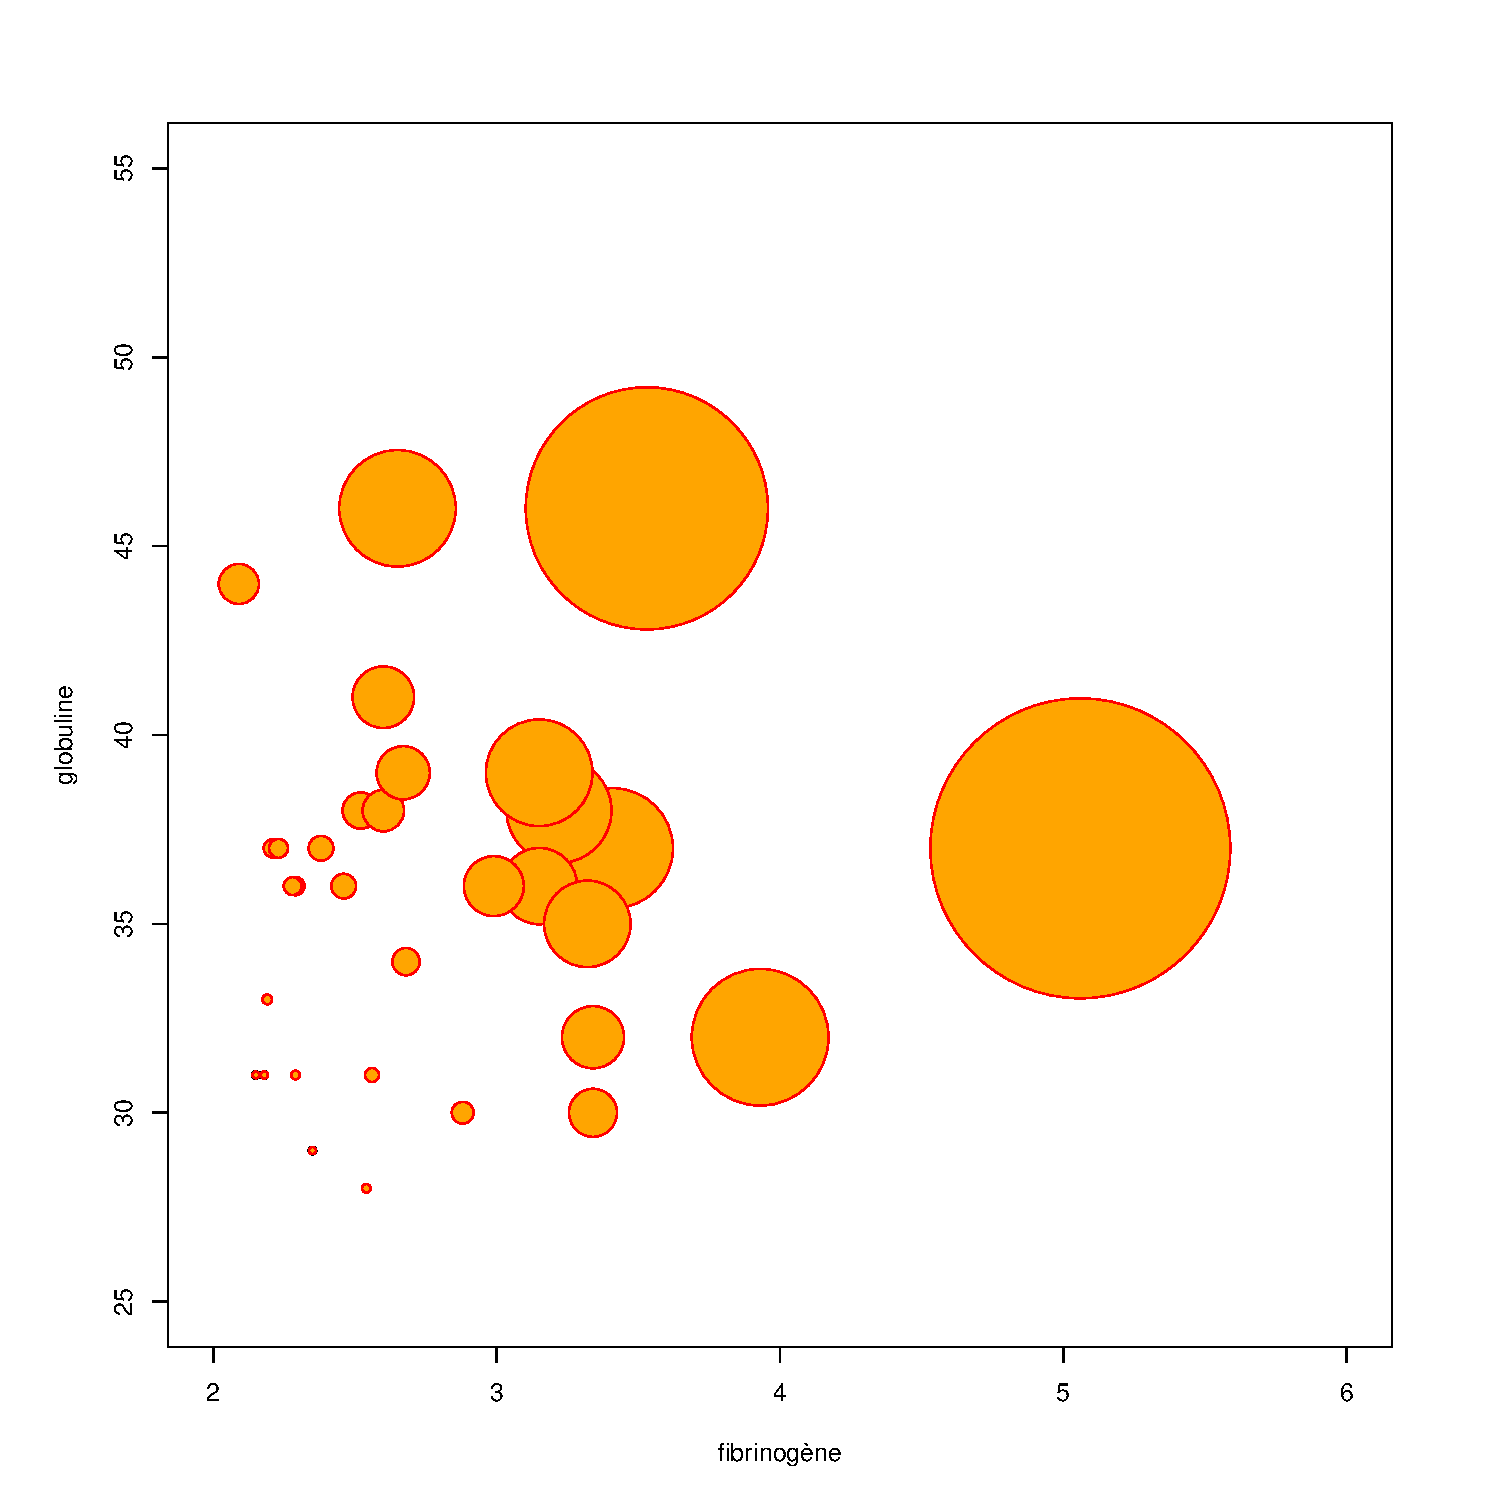
\includegraphics{pw1_VID_files/figure-pdf/unnamed-chunk-13-1.pdf}

}

\end{figure}

Nous pouvons dire que plus les variables ont des valeurs élevées
(fibrinogène et globuline) plus la probabilité semble élevée.

Q4B:

Nous pouvons calculer les corrélations avec le code suivant: Nous
constatons que toutes les valeurs sont très similaires bien que le
dataset soit très différent.

\begin{Shaded}
\begin{Highlighting}[]
\FunctionTok{data}\NormalTok{(anscombe)}



\NormalTok{correlation\_x1\_y1 }\OtherTok{\textless{}{-}} \FunctionTok{cor}\NormalTok{(anscombe}\SpecialCharTok{$}\NormalTok{x1, anscombe}\SpecialCharTok{$}\NormalTok{y1)}
\NormalTok{correlation\_x2\_y2 }\OtherTok{\textless{}{-}} \FunctionTok{cor}\NormalTok{(anscombe}\SpecialCharTok{$}\NormalTok{x2, anscombe}\SpecialCharTok{$}\NormalTok{y2)}
\NormalTok{correlation\_x3\_y3 }\OtherTok{\textless{}{-}} \FunctionTok{cor}\NormalTok{(anscombe}\SpecialCharTok{$}\NormalTok{x1, anscombe}\SpecialCharTok{$}\NormalTok{y3)}
\NormalTok{correlation\_x4\_y4 }\OtherTok{\textless{}{-}} \FunctionTok{cor}\NormalTok{(anscombe}\SpecialCharTok{$}\NormalTok{x4, anscombe}\SpecialCharTok{$}\NormalTok{y4)}

\FunctionTok{print}\NormalTok{(correlation\_x1\_y1)}
\end{Highlighting}
\end{Shaded}

\begin{verbatim}
[1] 0.8164205
\end{verbatim}

\begin{Shaded}
\begin{Highlighting}[]
\FunctionTok{print}\NormalTok{(correlation\_x2\_y2)}
\end{Highlighting}
\end{Shaded}

\begin{verbatim}
[1] 0.8162365
\end{verbatim}

\begin{Shaded}
\begin{Highlighting}[]
\FunctionTok{print}\NormalTok{(correlation\_x3\_y3)}
\end{Highlighting}
\end{Shaded}

\begin{verbatim}
[1] 0.8162867
\end{verbatim}

\begin{Shaded}
\begin{Highlighting}[]
\FunctionTok{print}\NormalTok{(correlation\_x4\_y4)}
\end{Highlighting}
\end{Shaded}

\begin{verbatim}
[1] 0.8165214
\end{verbatim}

Q4C:

\begin{Shaded}
\begin{Highlighting}[]
\NormalTok{anscombe}\FloatTok{.1}\OtherTok{\textless{}{-}}\FunctionTok{data.frame}\NormalTok{(}\AttributeTok{x1=}\NormalTok{anscombe}\SpecialCharTok{$}\NormalTok{x1, }\AttributeTok{x4=}\NormalTok{anscombe}\SpecialCharTok{$}\NormalTok{x4, }\AttributeTok{y1=}\NormalTok{anscombe}\SpecialCharTok{$}\NormalTok{y1, }
                       \AttributeTok{y2=}\NormalTok{anscombe}\SpecialCharTok{$}\NormalTok{y2, }\AttributeTok{y3=}\NormalTok{anscombe}\SpecialCharTok{$}\NormalTok{y3, }\AttributeTok{y4=}\NormalTok{anscombe}\SpecialCharTok{$}\NormalTok{y4)}
\end{Highlighting}
\end{Shaded}

Q4D:

\begin{Shaded}
\begin{Highlighting}[]
\FunctionTok{library}\NormalTok{(corrplot)}

\NormalTok{correlation\_matrix }\OtherTok{\textless{}{-}} \FunctionTok{cor}\NormalTok{(anscombe}\FloatTok{.1}\NormalTok{)}
\FunctionTok{corrplot.mixed}\NormalTok{(correlation\_matrix)}
\end{Highlighting}
\end{Shaded}

\begin{figure}[H]

{\centering 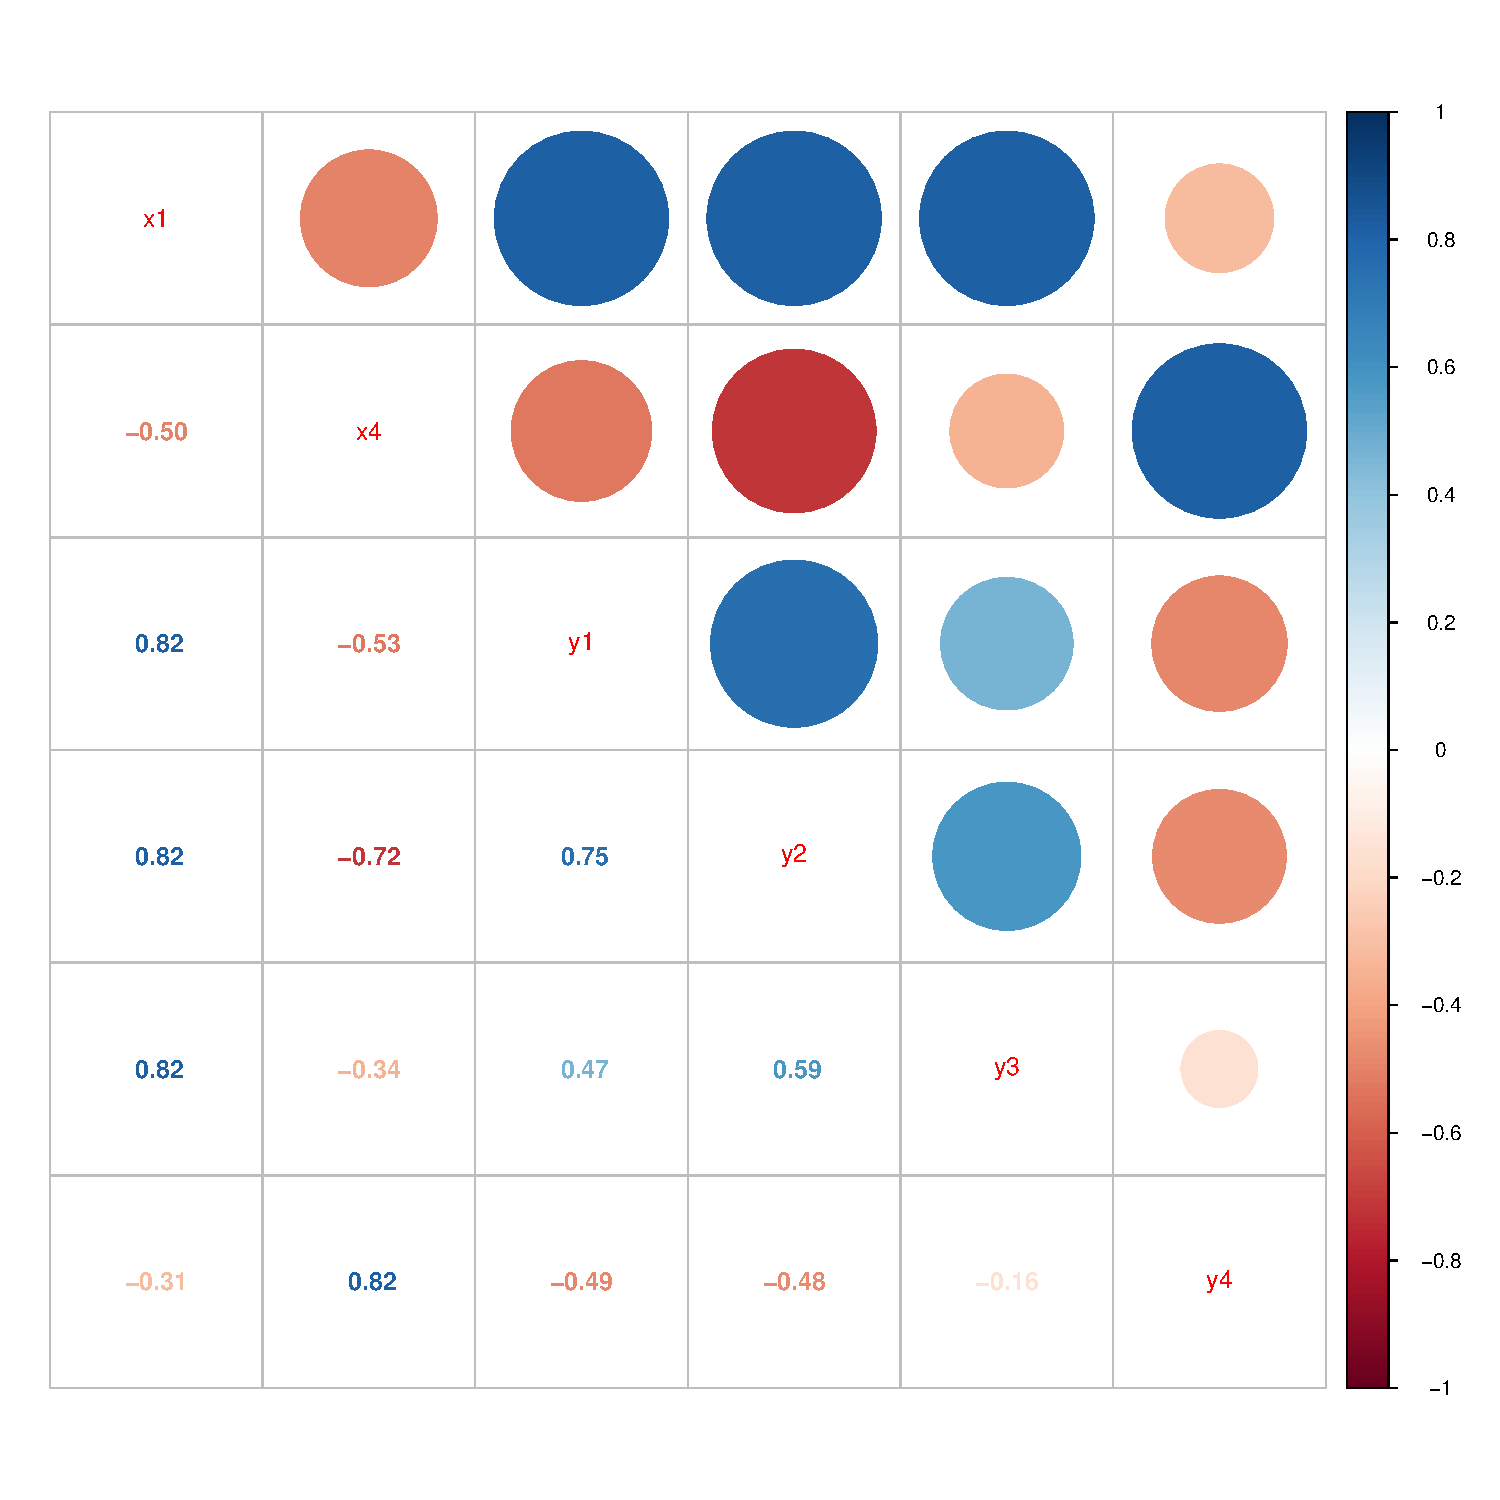
\includegraphics{pw1_VID_files/figure-pdf/unnamed-chunk-16-1.pdf}

}

\end{figure}

Q4E:

\begin{Shaded}
\begin{Highlighting}[]
\FunctionTok{library}\NormalTok{(corrr)}

\NormalTok{correlation\_matrix }\OtherTok{\textless{}{-}} \FunctionTok{correlate}\NormalTok{(anscombe}\FloatTok{.1}\NormalTok{)}
\FunctionTok{network\_plot}\NormalTok{(correlation\_matrix)}
\end{Highlighting}
\end{Shaded}

\begin{figure}[H]

{\centering 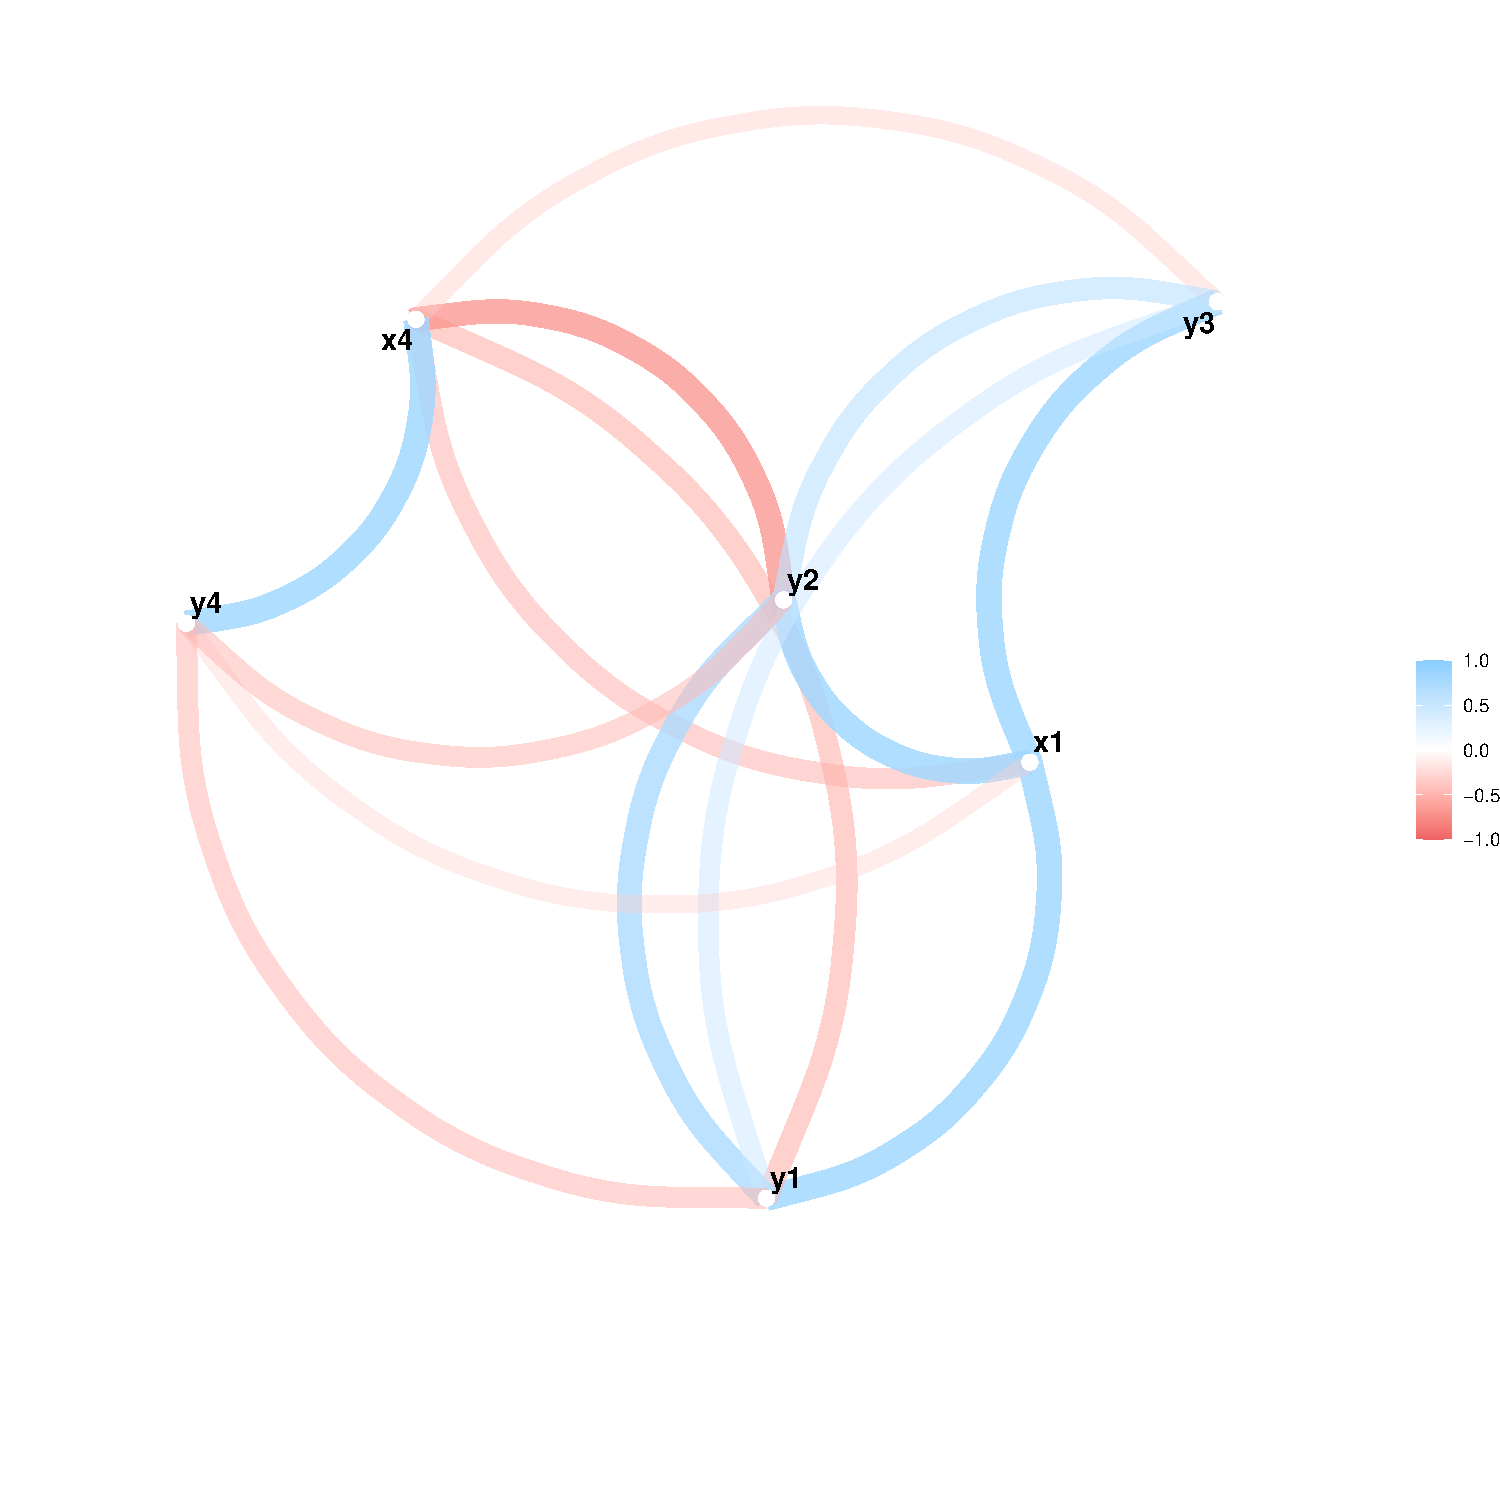
\includegraphics{pw1_VID_files/figure-pdf/unnamed-chunk-17-1.pdf}

}

\end{figure}

Q4F:

Nous pourrions envisager d'ajouter la `fit-line' ou droite de régression
afin de visualiser aussi où se trouvent les données par rapport à une
régression.

\begin{Shaded}
\begin{Highlighting}[]
\FunctionTok{library}\NormalTok{(ggplot2)}
\FunctionTok{library}\NormalTok{(GGally)}
\FunctionTok{library}\NormalTok{(GGally)}

\FunctionTok{theme\_set}\NormalTok{(}\FunctionTok{theme\_bw}\NormalTok{())}

\FunctionTok{ggpairs}\NormalTok{(anscombe}\FloatTok{.1}\NormalTok{,}
        \AttributeTok{lower=}\FunctionTok{list}\NormalTok{(}\AttributeTok{continuous=}\FunctionTok{wrap}\NormalTok{(}\StringTok{"points"}\NormalTok{, }\AttributeTok{alpha=}\FloatTok{0.8}\NormalTok{, }\AttributeTok{colour=}\StringTok{"\#FF8247"}\NormalTok{)),}
        \AttributeTok{aspect=}\StringTok{"iso"}\NormalTok{,}
        \AttributeTok{title=}\StringTok{"Séries de Francis Anscombe"}\NormalTok{)}
\end{Highlighting}
\end{Shaded}

\begin{figure}[H]

{\centering 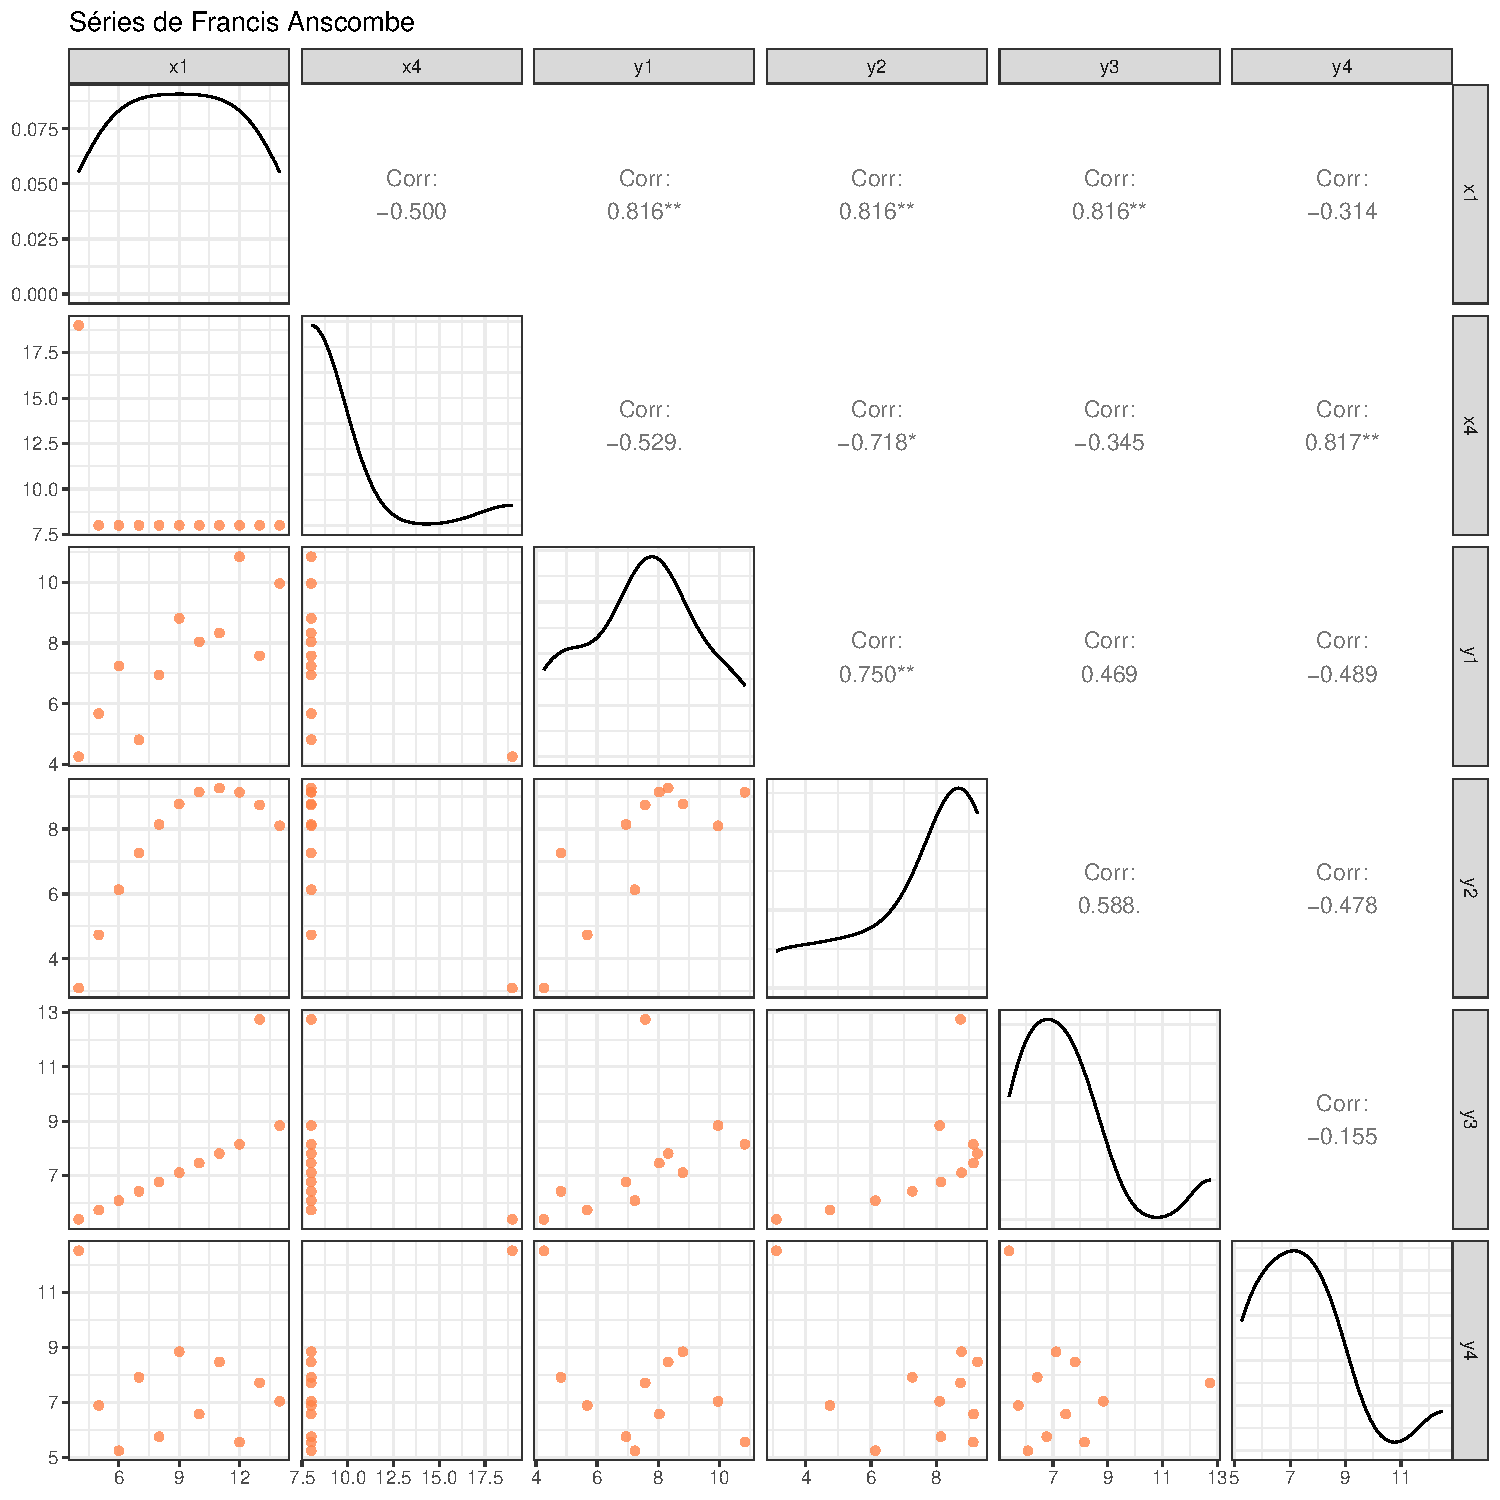
\includegraphics{pw1_VID_files/figure-pdf/unnamed-chunk-18-1.pdf}

}

\end{figure}

Q4G:

\begin{Shaded}
\begin{Highlighting}[]
\FunctionTok{library}\NormalTok{(ggplot2)}
\FunctionTok{library}\NormalTok{(GGally)}

\FunctionTok{par}\NormalTok{(}\AttributeTok{mfrow=}\FunctionTok{c}\NormalTok{(}\DecValTok{2}\NormalTok{, }\DecValTok{2}\NormalTok{),}\AttributeTok{pty=}\StringTok{"s"}\NormalTok{)}

\FunctionTok{plot}\NormalTok{(anscombe}\SpecialCharTok{$}\NormalTok{x1, anscombe}\SpecialCharTok{$}\NormalTok{y1, }\AttributeTok{pch=}\DecValTok{21}\NormalTok{, }\AttributeTok{bg=}\StringTok{"orange"}\NormalTok{, }\AttributeTok{xlab=}\StringTok{""}\NormalTok{, }\AttributeTok{ylab=}\StringTok{""}\NormalTok{, }\AttributeTok{xlim=}\FunctionTok{c}\NormalTok{(}\DecValTok{4}\NormalTok{, }\DecValTok{20}\NormalTok{),}

     \AttributeTok{ylim=}\FunctionTok{c}\NormalTok{(}\DecValTok{4}\NormalTok{, }\DecValTok{14}\NormalTok{))}

\FunctionTok{plot}\NormalTok{(anscombe}\SpecialCharTok{$}\NormalTok{x1, anscombe}\SpecialCharTok{$}\NormalTok{y2, }\AttributeTok{pch=}\DecValTok{21}\NormalTok{, }\AttributeTok{bg=}\StringTok{"orange"}\NormalTok{, }\AttributeTok{xlab=}\StringTok{""}\NormalTok{, }\AttributeTok{ylab=}\StringTok{""}\NormalTok{, }\AttributeTok{xlim=}\FunctionTok{c}\NormalTok{(}\DecValTok{4}\NormalTok{, }\DecValTok{20}\NormalTok{),}

     \AttributeTok{ylim=}\FunctionTok{c}\NormalTok{(}\DecValTok{4}\NormalTok{, }\DecValTok{14}\NormalTok{))}

\FunctionTok{plot}\NormalTok{(anscombe}\SpecialCharTok{$}\NormalTok{x1, anscombe}\SpecialCharTok{$}\NormalTok{y3, }\AttributeTok{pch=}\DecValTok{21}\NormalTok{, }\AttributeTok{bg=}\StringTok{"orange"}\NormalTok{, }\AttributeTok{xlab=}\StringTok{""}\NormalTok{, }\AttributeTok{ylab=}\StringTok{""}\NormalTok{, }\AttributeTok{xlim=}\FunctionTok{c}\NormalTok{(}\DecValTok{4}\NormalTok{, }\DecValTok{20}\NormalTok{),}

     \AttributeTok{ylim=}\FunctionTok{c}\NormalTok{(}\DecValTok{4}\NormalTok{, }\DecValTok{14}\NormalTok{))}

\FunctionTok{plot}\NormalTok{(anscombe}\SpecialCharTok{$}\NormalTok{x4, anscombe}\SpecialCharTok{$}\NormalTok{y4, }\AttributeTok{pch=}\DecValTok{21}\NormalTok{, }\AttributeTok{bg=}\StringTok{"orange"}\NormalTok{, }\AttributeTok{xlab=}\StringTok{""}\NormalTok{, }\AttributeTok{ylab=}\StringTok{""}\NormalTok{, }\AttributeTok{xlim=}\FunctionTok{c}\NormalTok{(}\DecValTok{4}\NormalTok{, }\DecValTok{20}\NormalTok{),}

     \AttributeTok{ylim=}\FunctionTok{c}\NormalTok{(}\DecValTok{4}\NormalTok{, }\DecValTok{14}\NormalTok{))}

\FunctionTok{par}\NormalTok{(}\AttributeTok{mfrow=}\FunctionTok{c}\NormalTok{(}\DecValTok{1}\NormalTok{, }\DecValTok{1}\NormalTok{))}

\FunctionTok{legend}\NormalTok{(}\FloatTok{9.5}\NormalTok{, }\DecValTok{9}\NormalTok{, }\StringTok{"r = 0.82"}\NormalTok{, }\AttributeTok{bty=}\StringTok{"n"}\NormalTok{)}
\end{Highlighting}
\end{Shaded}

\begin{figure}[H]

{\centering 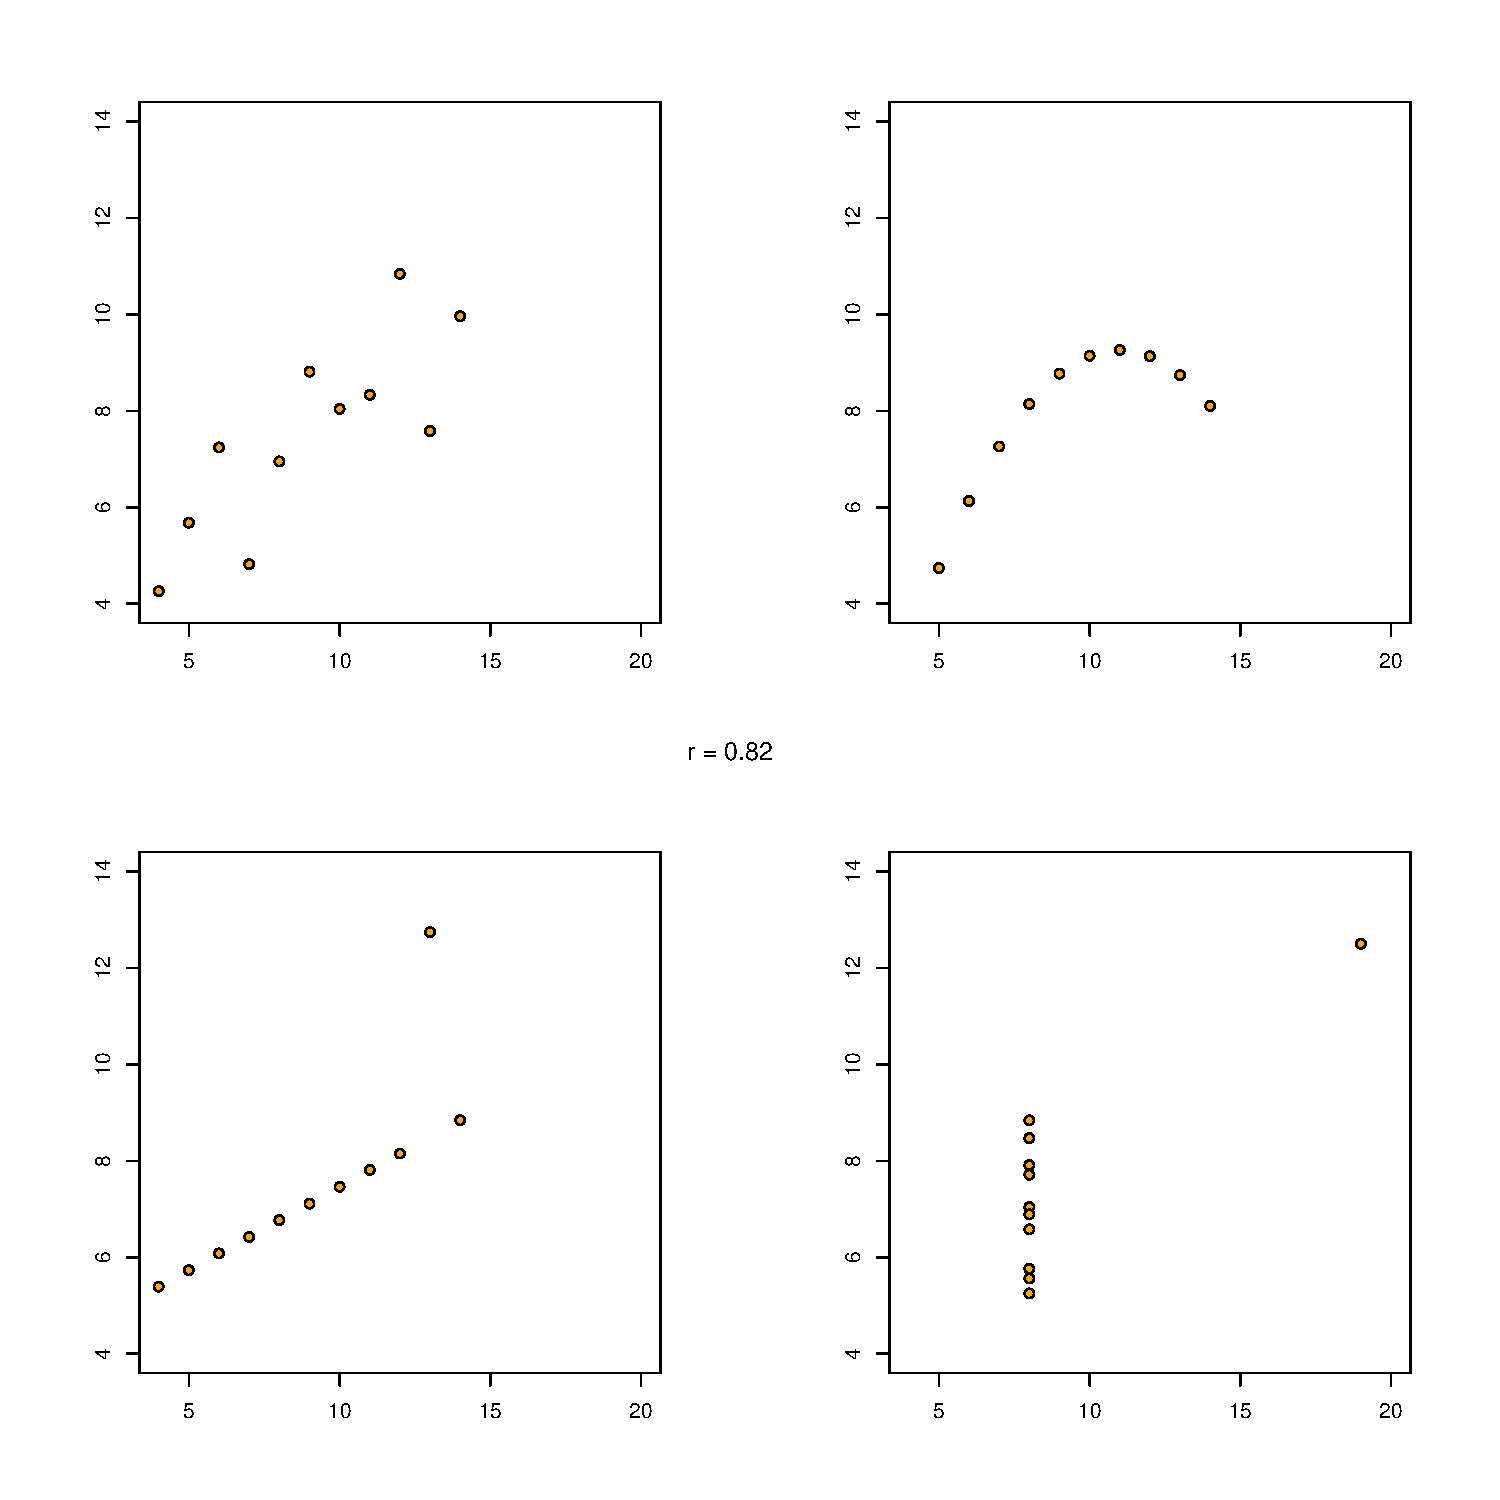
\includegraphics{pw1_VID_files/figure-pdf/unnamed-chunk-19-1.pdf}

}

\end{figure}

Q4H:

Le premier graphe (corrplot.mixed) nous permet de visualiser les valeurs
de corrélation ainsi qu'une représentation visuelle à l'aide de points.
Et ceci, entre les paires de variable données.

Le deuxième graphe (network plot) nous permet d'uniquement comparer les
corrélation de manière visuelle. Nous disposons uniquement du graphe et
ses connexions avec les magnitudes de celles-ci. Un graphe intéressant
si nous désirons mettre en évidence uniquement les relations entre les
variables sans surcharger la visualisation de valeurs.

Le troisième graphe en matrice (scatter plot matrix) nous permet de voir
à la fois la valeur du R\^{}2 mais aussi le scatter plot de la
combinaison de variables. la diagonale nous informe de la distribution
des données. Nous devons regarder à quelle cellule correspond chaque
paire valeur-scatter-plot ce qui peut être mal adapté pour une
compréhension instantanée des données.

Nous pourrions souhaiter afficher la corrélation directement dans la
cellule et afficher un deuxième scatter-plot avec la même combinaison de
variable mais de manière à inverser les abscisses et ordonnées.

Le dernier graphe en matrice de 4 sous-graphes est intéressant par sa
clarté. En effet, en affichant le R\^{}2 au centre il est facilement
compréhensible que cette information concerne tous les graphes.

Q5A:

\begin{Shaded}
\begin{Highlighting}[]
\FunctionTok{library}\NormalTok{(skimr)}
\FunctionTok{library}\NormalTok{(ggplot2)}
\FunctionTok{library}\NormalTok{(palmerpenguins)}

\FunctionTok{skim}\NormalTok{(penguins)}
\end{Highlighting}
\end{Shaded}

\begin{longtable}[]{@{}ll@{}}
\caption{Data summary}\tabularnewline
\toprule\noalign{}
\endfirsthead
\endhead
\bottomrule\noalign{}
\endlastfoot
Name & penguins \\
Number of rows & 344 \\
Number of columns & 8 \\
\_\_\_\_\_\_\_\_\_\_\_\_\_\_\_\_\_\_\_\_\_\_\_ & \\
Column type frequency: & \\
factor & 3 \\
numeric & 5 \\
\_\_\_\_\_\_\_\_\_\_\_\_\_\_\_\_\_\_\_\_\_\_\_\_ & \\
Group variables & None \\
\end{longtable}

\textbf{Variable type: factor}

\begin{longtable}[]{@{}
  >{\raggedright\arraybackslash}p{(\columnwidth - 10\tabcolsep) * \real{0.1687}}
  >{\raggedleft\arraybackslash}p{(\columnwidth - 10\tabcolsep) * \real{0.1205}}
  >{\raggedleft\arraybackslash}p{(\columnwidth - 10\tabcolsep) * \real{0.1687}}
  >{\raggedright\arraybackslash}p{(\columnwidth - 10\tabcolsep) * \real{0.0964}}
  >{\raggedleft\arraybackslash}p{(\columnwidth - 10\tabcolsep) * \real{0.1084}}
  >{\raggedright\arraybackslash}p{(\columnwidth - 10\tabcolsep) * \real{0.3373}}@{}}
\toprule\noalign{}
\begin{minipage}[b]{\linewidth}\raggedright
skim\_variable
\end{minipage} & \begin{minipage}[b]{\linewidth}\raggedleft
n\_missing
\end{minipage} & \begin{minipage}[b]{\linewidth}\raggedleft
complete\_rate
\end{minipage} & \begin{minipage}[b]{\linewidth}\raggedright
ordered
\end{minipage} & \begin{minipage}[b]{\linewidth}\raggedleft
n\_unique
\end{minipage} & \begin{minipage}[b]{\linewidth}\raggedright
top\_counts
\end{minipage} \\
\midrule\noalign{}
\endhead
\bottomrule\noalign{}
\endlastfoot
species & 0 & 1.00 & FALSE & 3 & Ade: 152, Gen: 124, Chi: 68 \\
island & 0 & 1.00 & FALSE & 3 & Bis: 168, Dre: 124, Tor: 52 \\
sex & 11 & 0.97 & FALSE & 2 & mal: 168, fem: 165 \\
\end{longtable}

\textbf{Variable type: numeric}

\begin{longtable}[]{@{}
  >{\raggedright\arraybackslash}p{(\columnwidth - 20\tabcolsep) * \real{0.1800}}
  >{\raggedleft\arraybackslash}p{(\columnwidth - 20\tabcolsep) * \real{0.1000}}
  >{\raggedleft\arraybackslash}p{(\columnwidth - 20\tabcolsep) * \real{0.1400}}
  >{\raggedleft\arraybackslash}p{(\columnwidth - 20\tabcolsep) * \real{0.0800}}
  >{\raggedleft\arraybackslash}p{(\columnwidth - 20\tabcolsep) * \real{0.0700}}
  >{\raggedleft\arraybackslash}p{(\columnwidth - 20\tabcolsep) * \real{0.0700}}
  >{\raggedleft\arraybackslash}p{(\columnwidth - 20\tabcolsep) * \real{0.0800}}
  >{\raggedleft\arraybackslash}p{(\columnwidth - 20\tabcolsep) * \real{0.0800}}
  >{\raggedleft\arraybackslash}p{(\columnwidth - 20\tabcolsep) * \real{0.0700}}
  >{\raggedleft\arraybackslash}p{(\columnwidth - 20\tabcolsep) * \real{0.0700}}
  >{\raggedright\arraybackslash}p{(\columnwidth - 20\tabcolsep) * \real{0.0600}}@{}}
\toprule\noalign{}
\begin{minipage}[b]{\linewidth}\raggedright
skim\_variable
\end{minipage} & \begin{minipage}[b]{\linewidth}\raggedleft
n\_missing
\end{minipage} & \begin{minipage}[b]{\linewidth}\raggedleft
complete\_rate
\end{minipage} & \begin{minipage}[b]{\linewidth}\raggedleft
mean
\end{minipage} & \begin{minipage}[b]{\linewidth}\raggedleft
sd
\end{minipage} & \begin{minipage}[b]{\linewidth}\raggedleft
p0
\end{minipage} & \begin{minipage}[b]{\linewidth}\raggedleft
p25
\end{minipage} & \begin{minipage}[b]{\linewidth}\raggedleft
p50
\end{minipage} & \begin{minipage}[b]{\linewidth}\raggedleft
p75
\end{minipage} & \begin{minipage}[b]{\linewidth}\raggedleft
p100
\end{minipage} & \begin{minipage}[b]{\linewidth}\raggedright
hist
\end{minipage} \\
\midrule\noalign{}
\endhead
\bottomrule\noalign{}
\endlastfoot
bill\_length\_mm & 2 & 0.99 & 43.92 & 5.46 & 32.1 & 39.23 & 44.45 & 48.5
& 59.6 & ▃▇▇▆▁ \\
bill\_depth\_mm & 2 & 0.99 & 17.15 & 1.97 & 13.1 & 15.60 & 17.30 & 18.7
& 21.5 & ▅▅▇▇▂ \\
flipper\_length\_mm & 2 & 0.99 & 200.92 & 14.06 & 172.0 & 190.00 &
197.00 & 213.0 & 231.0 & ▂▇▃▅▂ \\
body\_mass\_g & 2 & 0.99 & 4201.75 & 801.95 & 2700.0 & 3550.00 & 4050.00
& 4750.0 & 6300.0 & ▃▇▆▃▂ \\
year & 0 & 1.00 & 2008.03 & 0.82 & 2007.0 & 2007.00 & 2008.00 & 2009.0 &
2009.0 & ▇▁▇▁▇ \\
\end{longtable}

Q5B:

Nous nous apercevons que la variable `sex' a 11 valeurs manquantes.

Q5C:

L'espèce la plus représentée comme nous indique le code ci-dessous est
l'Adélie.

\begin{Shaded}
\begin{Highlighting}[]
\FunctionTok{print}\NormalTok{(}\FunctionTok{table}\NormalTok{(penguins}\SpecialCharTok{$}\NormalTok{species))}
\end{Highlighting}
\end{Shaded}

\begin{verbatim}

   Adelie Chinstrap    Gentoo 
      152        68       124 
\end{verbatim}

Q5D:

En calculant le coefficient de Pearson sans les NA nous obtenons un 65.6
\% de corrélation entre ces deux paramètres. Ce n'est pas significatif
donc nous pouvons affirmer que le corrélation est faible.

\begin{Shaded}
\begin{Highlighting}[]
\FunctionTok{print}\NormalTok{(}\FunctionTok{cor}\NormalTok{(penguins}\SpecialCharTok{$}\NormalTok{flipper\_length\_mm, penguins}\SpecialCharTok{$}\NormalTok{bill\_length\_mm, }\AttributeTok{use=}\StringTok{"complete.obs"}\NormalTok{ ))}
\end{Highlighting}
\end{Shaded}

\begin{verbatim}
[1] 0.6561813
\end{verbatim}

\begin{Shaded}
\begin{Highlighting}[]
\FunctionTok{library}\NormalTok{(skimr)}
\FunctionTok{library}\NormalTok{(ggplot2)}
\FunctionTok{library}\NormalTok{(palmerpenguins)}

\FunctionTok{ggplot}\NormalTok{(}\AttributeTok{data =}\NormalTok{ penguins, }\FunctionTok{aes}\NormalTok{(}\AttributeTok{x =}\NormalTok{ flipper\_length\_mm, }\AttributeTok{y =}\NormalTok{ bill\_length\_mm)) }\SpecialCharTok{+}
  \FunctionTok{geom\_point}\NormalTok{(}\FunctionTok{aes}\NormalTok{(}\AttributeTok{color =}\NormalTok{ species, }\AttributeTok{shape =}\NormalTok{ species), }\AttributeTok{size =} \DecValTok{3}\NormalTok{, }\AttributeTok{alpha =} \FloatTok{0.8}\NormalTok{) }\SpecialCharTok{+}
  \FunctionTok{scale\_color\_manual}\NormalTok{(}\AttributeTok{values =} \FunctionTok{c}\NormalTok{(}\StringTok{"darkorange"}\NormalTok{,}\StringTok{"purple"}\NormalTok{,}\StringTok{"cyan4"}\NormalTok{)) }\SpecialCharTok{+}
  \FunctionTok{labs}\NormalTok{(}\AttributeTok{title =} \StringTok{"Taille des manchots, Palmer Station LTER"}\NormalTok{,}
  \AttributeTok{subtitle =} \StringTok{"Longueur des nageoires et longueur du bec chez les manchots Adelie,    Chinstrap et de Gentoo"}\NormalTok{,)}
\end{Highlighting}
\end{Shaded}

\begin{figure}[H]

{\centering 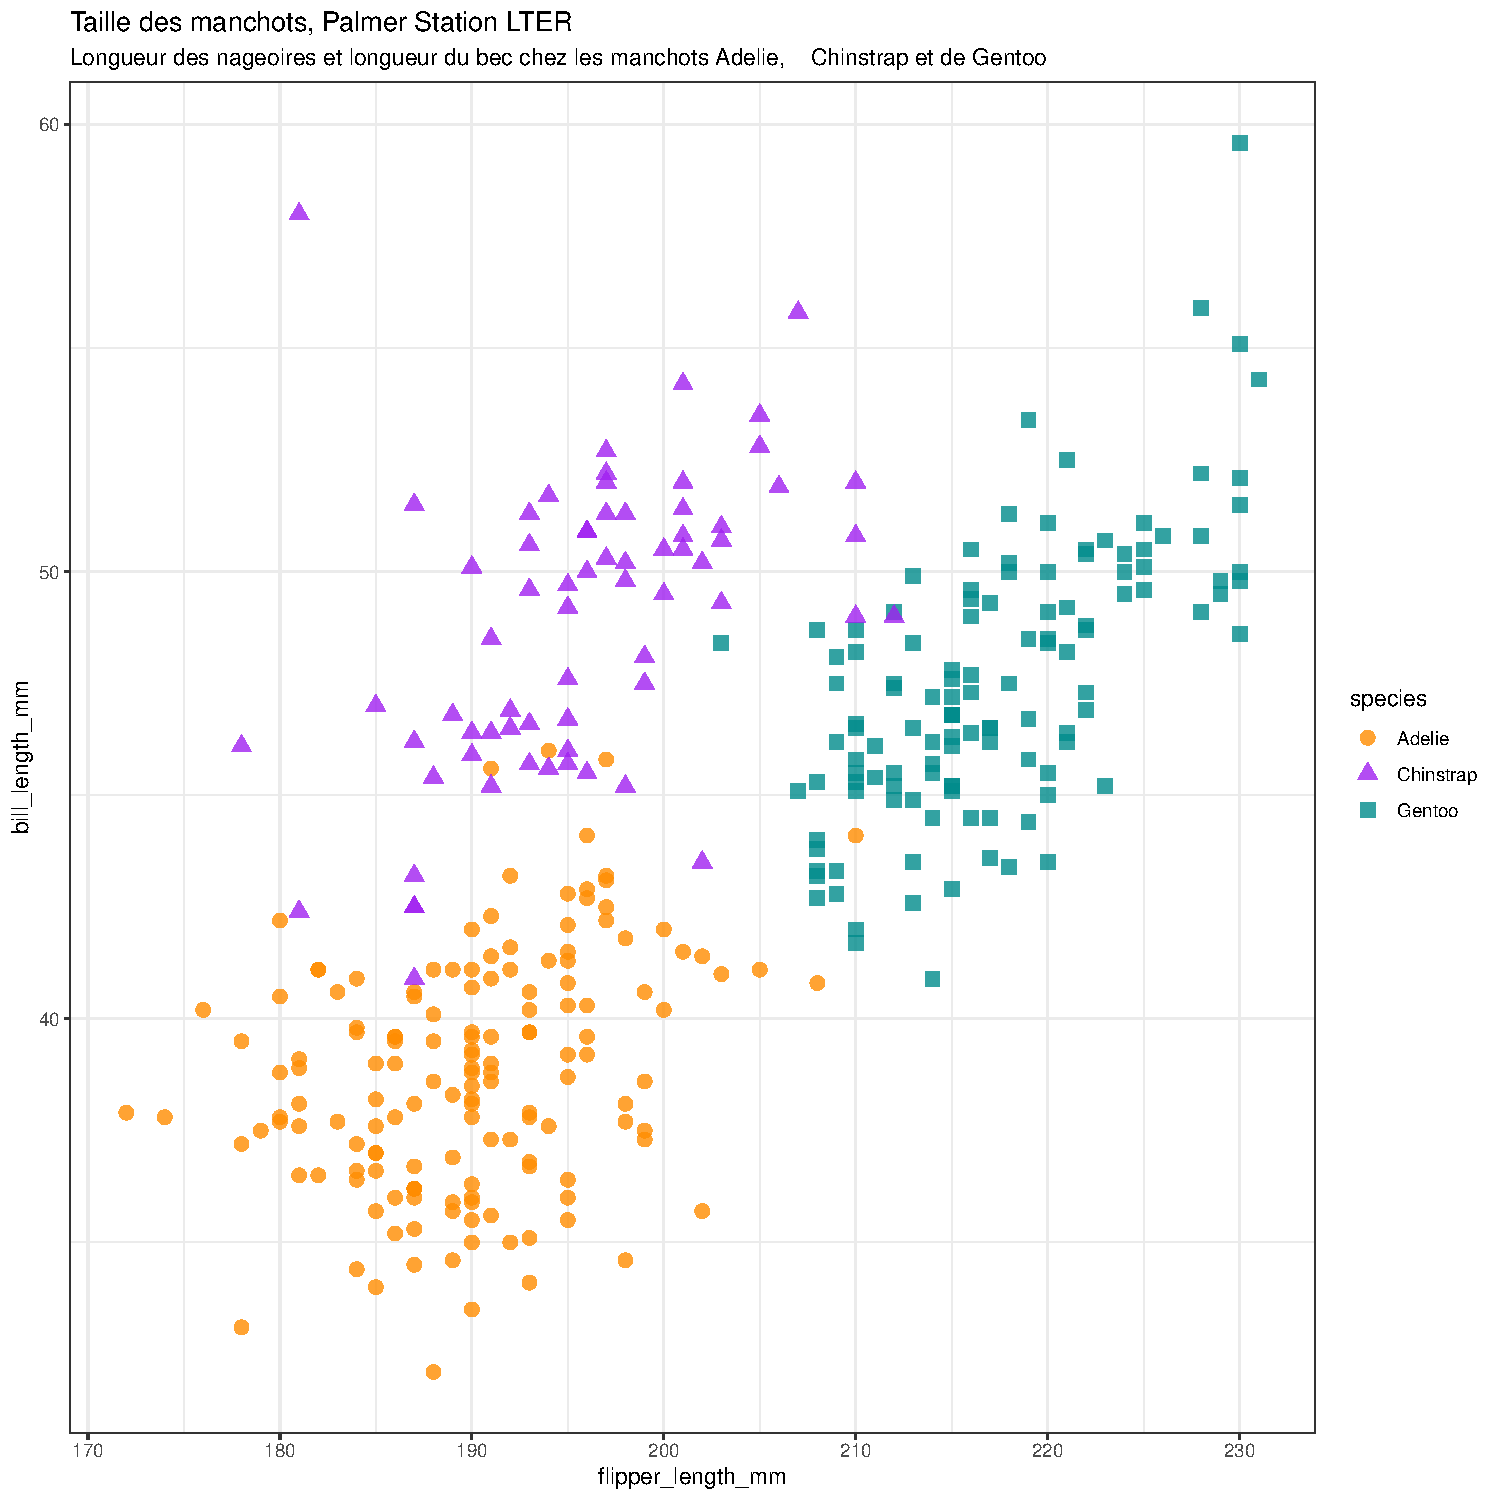
\includegraphics{pw1_VID_files/figure-pdf/unnamed-chunk-23-1.pdf}

}

\end{figure}

Q5E:

Nous observons un Chinstrap avec une longueur de nageoire anormalement
longue (180mm) et un bec de \textasciitilde57mm). Le reste des donnée
semble relativement régulier.

Q5F:

Nous pourrions envisager de discriminer le Chinstrap en prenant par
exemple la valeur de 205mm pour la longueur des nageoires.

Q5G:

Voir Q5D:

Q5H:

En modifiant le paramètre shape nous pouvons visualiser les iles avec la
forme.

Les manchots de Gentoo vivent exclusivement sur Biscoe.

\begin{Shaded}
\begin{Highlighting}[]
\FunctionTok{library}\NormalTok{(skimr)}
\FunctionTok{library}\NormalTok{(ggplot2)}
\FunctionTok{library}\NormalTok{(palmerpenguins)}

\FunctionTok{ggplot}\NormalTok{(}\AttributeTok{data =}\NormalTok{ penguins, }\FunctionTok{aes}\NormalTok{(}\AttributeTok{x =}\NormalTok{ flipper\_length\_mm, }\AttributeTok{y =}\NormalTok{ bill\_length\_mm)) }\SpecialCharTok{+}
  \FunctionTok{geom\_point}\NormalTok{(}\FunctionTok{aes}\NormalTok{(}\AttributeTok{color =}\NormalTok{ species, }\AttributeTok{shape =}\NormalTok{ island), }\AttributeTok{size =} \DecValTok{3}\NormalTok{, }\AttributeTok{alpha =} \FloatTok{0.8}\NormalTok{) }\SpecialCharTok{+}
  \FunctionTok{scale\_color\_manual}\NormalTok{(}\AttributeTok{values =} \FunctionTok{c}\NormalTok{(}\StringTok{"darkorange"}\NormalTok{,}\StringTok{"purple"}\NormalTok{,}\StringTok{"cyan4"}\NormalTok{)) }\SpecialCharTok{+}
  \FunctionTok{labs}\NormalTok{(}\AttributeTok{title =} \StringTok{"Taille des manchots, Palmer Station LTER"}\NormalTok{,}
  \AttributeTok{subtitle =} \StringTok{"Longueur des nageoires et longueur du bec chez les manchots Adelie,    Chinstrap et de Gentoo"}\NormalTok{,)}
\end{Highlighting}
\end{Shaded}

\begin{figure}[H]

{\centering 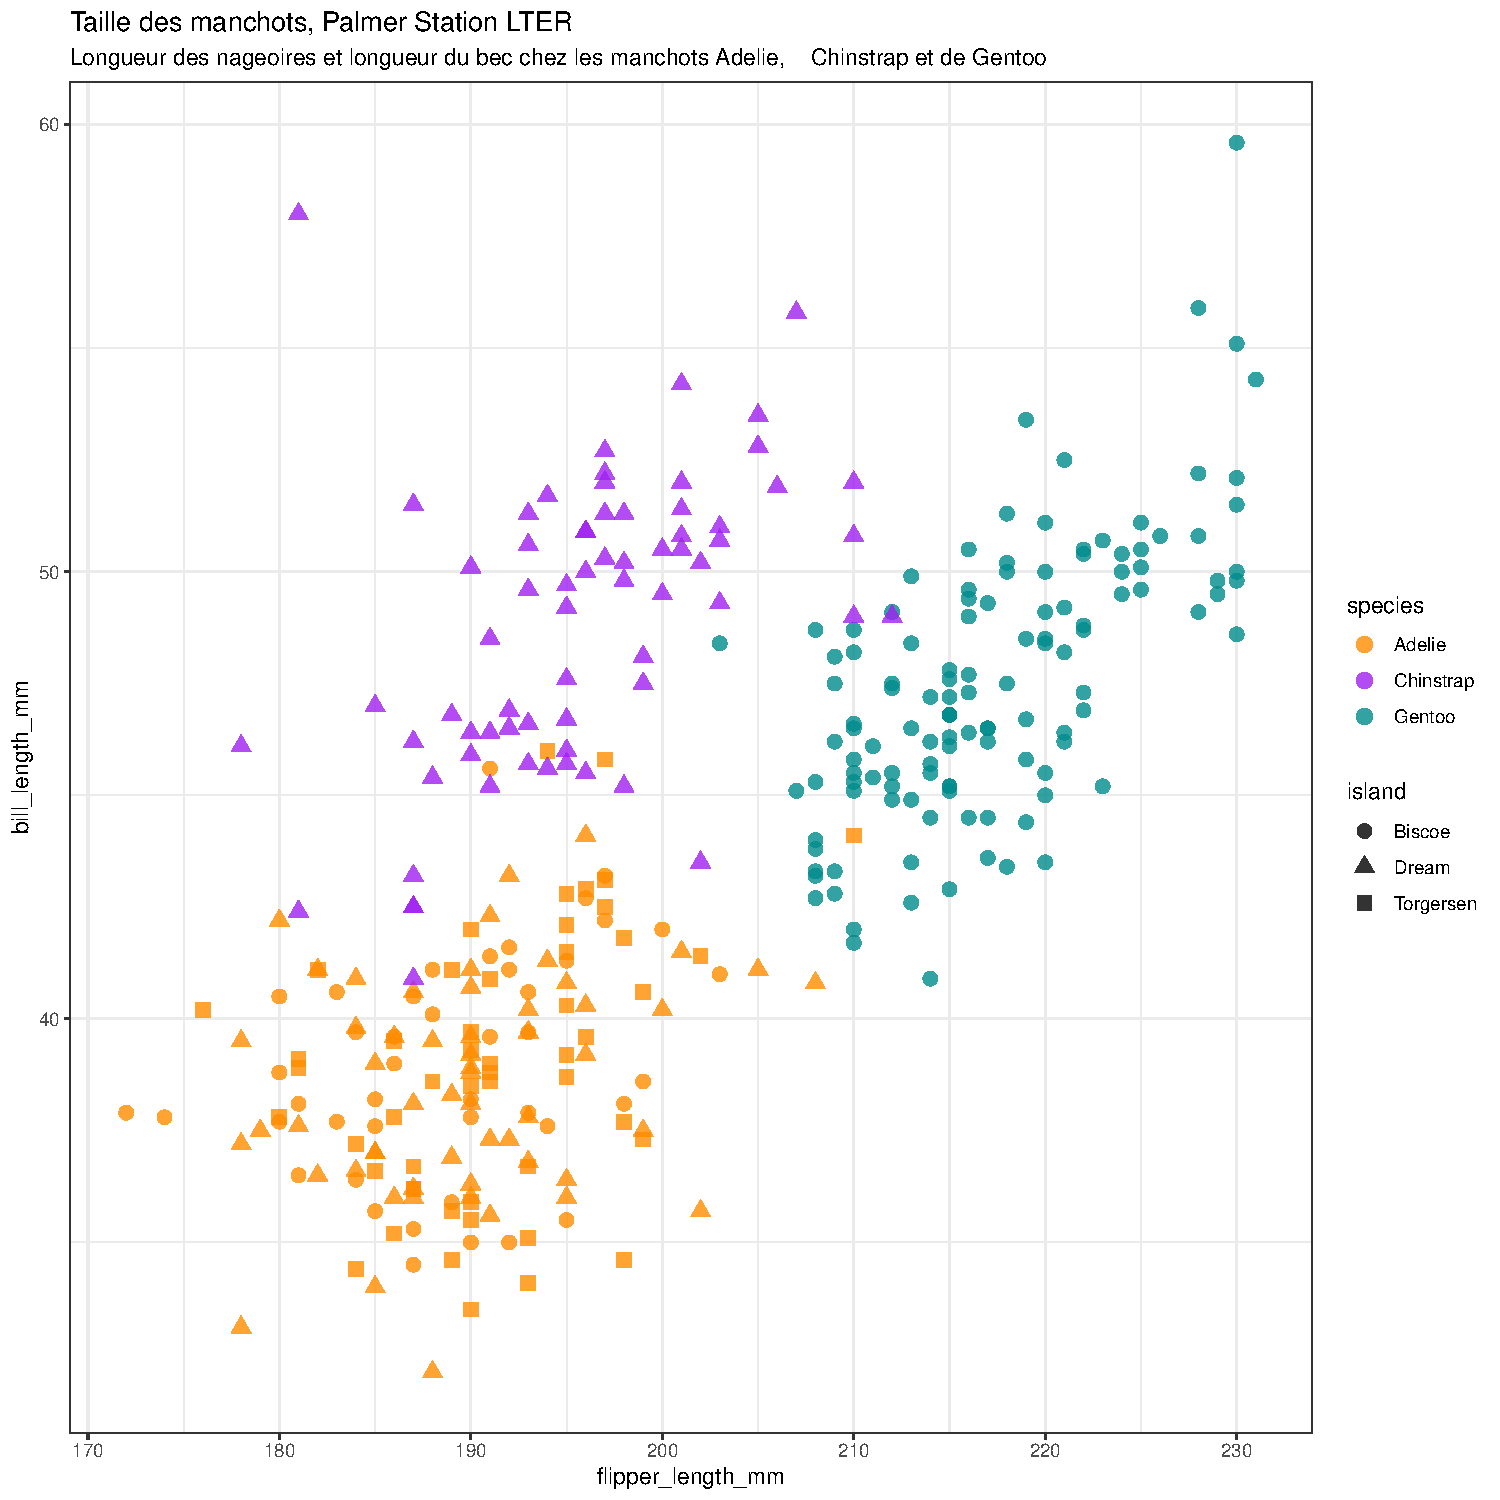
\includegraphics{pw1_VID_files/figure-pdf/unnamed-chunk-24-1.pdf}

}

\end{figure}

Q5I:

\begin{Shaded}
\begin{Highlighting}[]
\FunctionTok{ggplot}\NormalTok{(penguins, }\FunctionTok{aes}\NormalTok{(}\AttributeTok{x =}\NormalTok{ island, }\AttributeTok{y =}\NormalTok{ species, }\AttributeTok{color =}\NormalTok{ species)) }\SpecialCharTok{+}
  \FunctionTok{geom\_jitter}\NormalTok{(}\AttributeTok{size =} \DecValTok{3}\NormalTok{) }\SpecialCharTok{+} 
  \FunctionTok{scale\_color\_manual}\NormalTok{(}\AttributeTok{values =} \FunctionTok{c}\NormalTok{(}\StringTok{"darkorange"}\NormalTok{,}\StringTok{"purple"}\NormalTok{,}\StringTok{"cyan4"}\NormalTok{)) }\SpecialCharTok{+}
  \FunctionTok{labs}\NormalTok{(}\AttributeTok{x =} \StringTok{"Iles"}\NormalTok{,}
       \AttributeTok{y =} \StringTok{"Espèce de manchots"}\NormalTok{,}
       \AttributeTok{color =} \StringTok{"Espèce de manchots"}\NormalTok{)}
\end{Highlighting}
\end{Shaded}

\begin{figure}[H]

{\centering 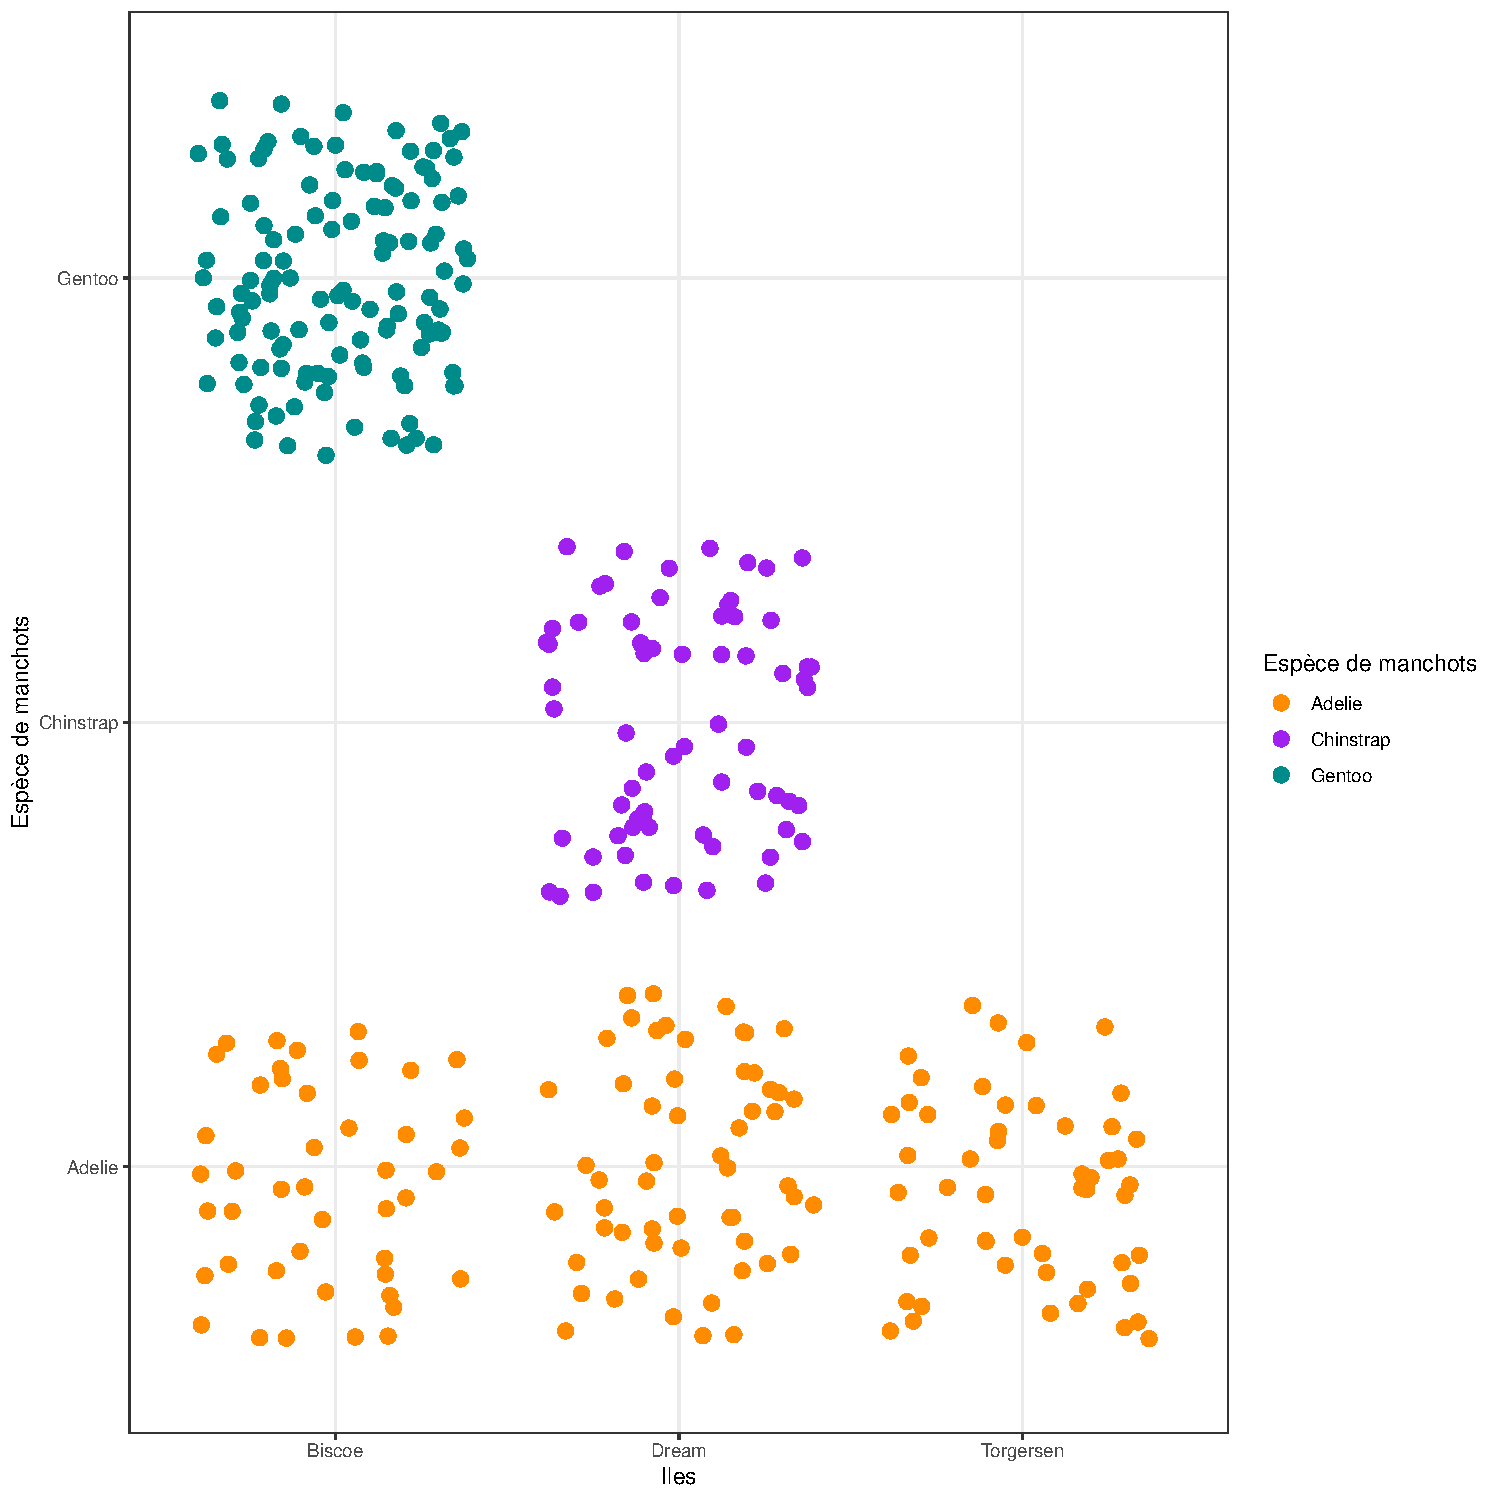
\includegraphics{pw1_VID_files/figure-pdf/unnamed-chunk-25-1.pdf}

}

\end{figure}

Q5J:

\begin{Shaded}
\begin{Highlighting}[]
\FunctionTok{library}\NormalTok{(ggplot2)}
\FunctionTok{library}\NormalTok{(palmerpenguins)}

\FunctionTok{ggplot}\NormalTok{(}\AttributeTok{data =}\NormalTok{ penguins, }\FunctionTok{aes}\NormalTok{(}\AttributeTok{x =}\NormalTok{ flipper\_length\_mm, }\AttributeTok{y =}\NormalTok{ bill\_length\_mm)) }\SpecialCharTok{+}
  \FunctionTok{geom\_point}\NormalTok{(}\FunctionTok{aes}\NormalTok{(}\AttributeTok{color =}\NormalTok{ sex), }\AttributeTok{size =} \DecValTok{5}\NormalTok{, }\AttributeTok{alpha =} \FloatTok{0.5}\NormalTok{) }\SpecialCharTok{+}
  \FunctionTok{scale\_color\_manual}\NormalTok{(}\AttributeTok{values =} \FunctionTok{c}\NormalTok{(}\StringTok{"red"}\NormalTok{, }\StringTok{"blue"}\NormalTok{, }\StringTok{"grey"}\NormalTok{)) }\SpecialCharTok{+}
  \FunctionTok{labs}\NormalTok{(}\AttributeTok{title =} \StringTok{"Taille des manchots, Palmer Station LTER"}\NormalTok{,}
       \AttributeTok{x =} \StringTok{"Longueur des nageoires (mm)"}\NormalTok{,}
       \AttributeTok{y =} \StringTok{"Longueur du bec (mm)"}\NormalTok{,}
       \AttributeTok{color =} \StringTok{"Espèce"}\NormalTok{,}
       \AttributeTok{shape =} \StringTok{"Sexe"}\NormalTok{) }\SpecialCharTok{+}
  \FunctionTok{facet\_wrap}\NormalTok{(}\SpecialCharTok{\textasciitilde{}}\NormalTok{species, }\AttributeTok{ncol =} \DecValTok{3}\NormalTok{)}
\end{Highlighting}
\end{Shaded}

\begin{figure}[H]

{\centering 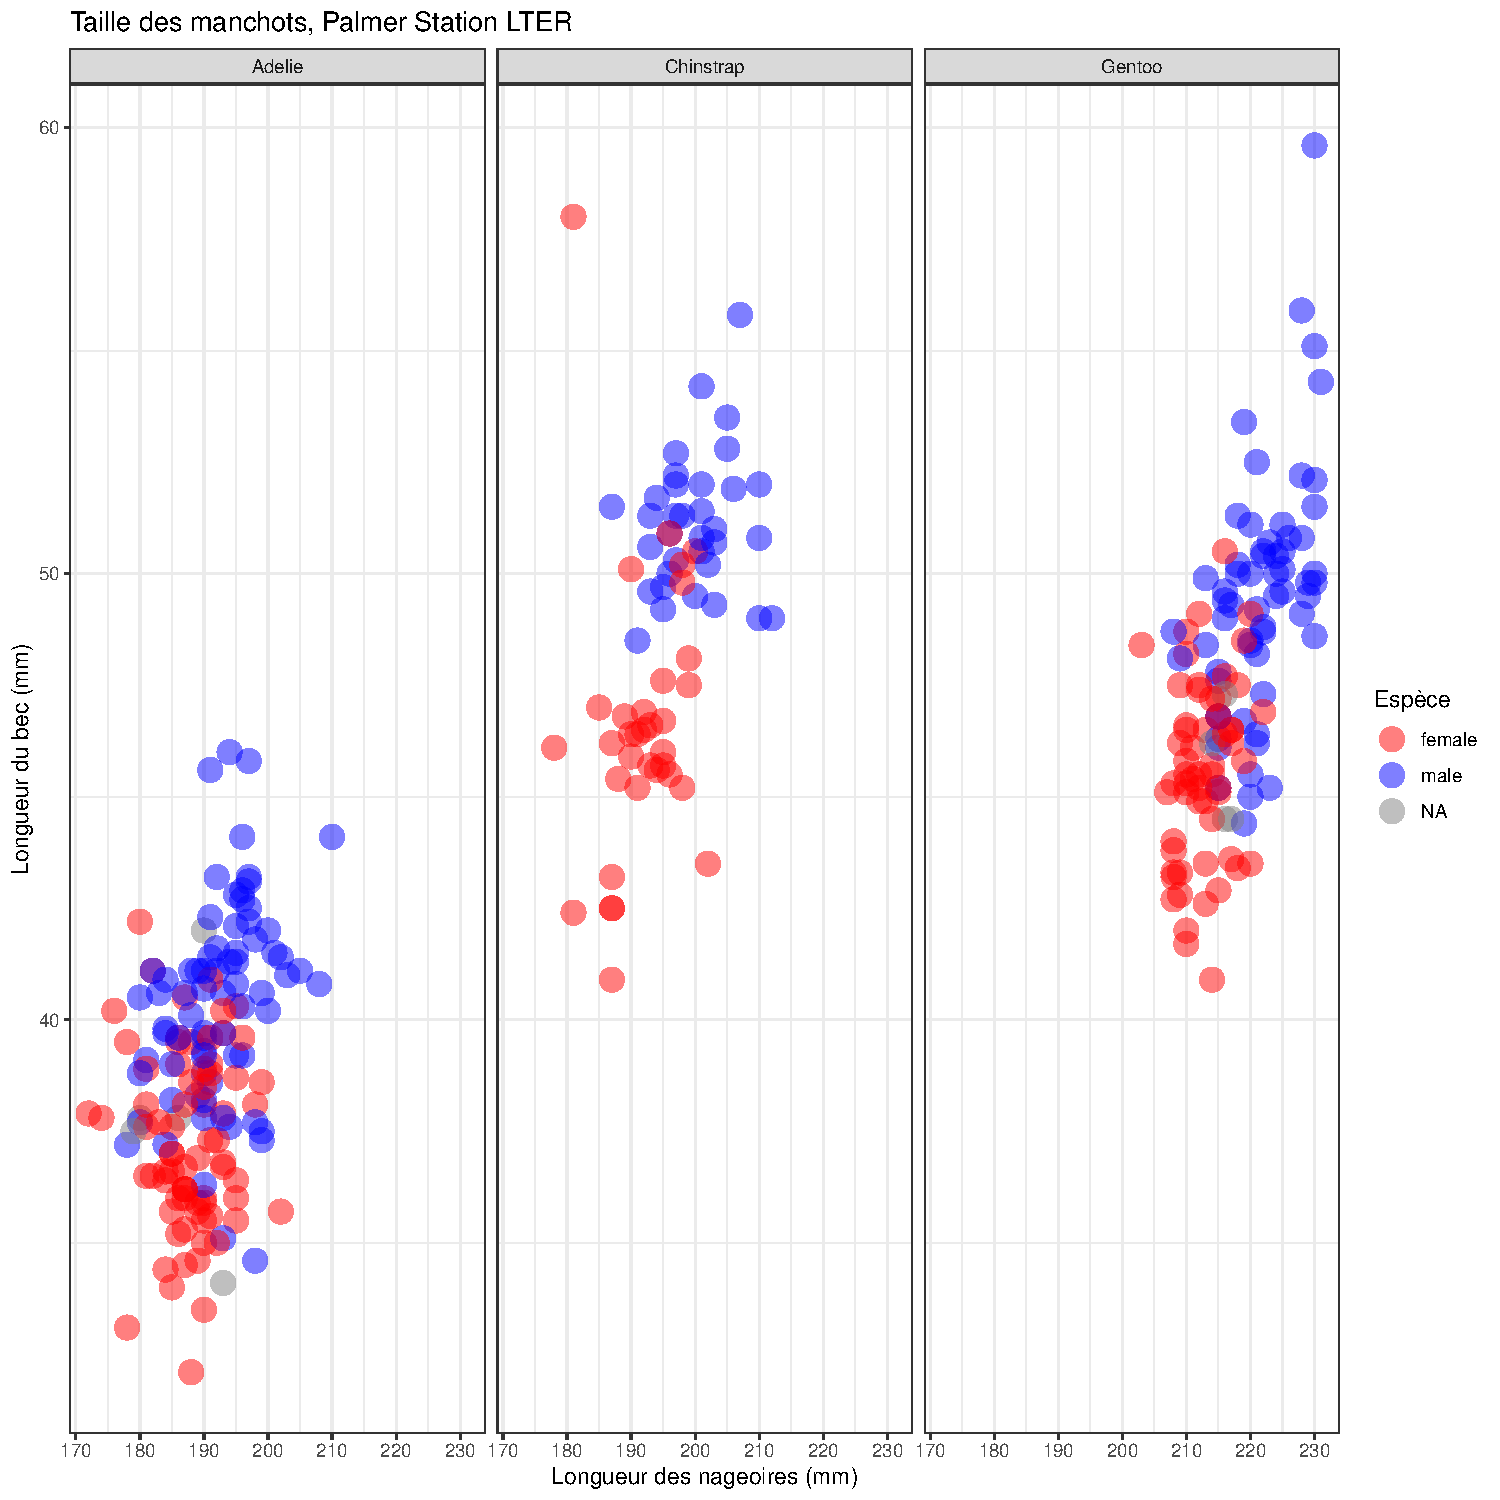
\includegraphics{pw1_VID_files/figure-pdf/unnamed-chunk-26-1.pdf}

}

\end{figure}

Q6A:

\begin{Shaded}
\begin{Highlighting}[]
\NormalTok{grant }\OtherTok{\textless{}{-}} \FunctionTok{read.csv}\NormalTok{(}\StringTok{"isc\_grants.csv"}\NormalTok{)}
\end{Highlighting}
\end{Shaded}

Q6B:

\begin{Shaded}
\begin{Highlighting}[]
\FunctionTok{library}\NormalTok{(ggplot2)}
\FunctionTok{library}\NormalTok{(treemapify)}
\FunctionTok{library}\NormalTok{(camcorder)}


\NormalTok{grant }\OtherTok{\textless{}{-}} \FunctionTok{read.csv}\NormalTok{(}\StringTok{"isc\_grants.csv"}\NormalTok{)}

\NormalTok{pal }\OtherTok{\textless{}{-}} \FunctionTok{c}\NormalTok{(}\StringTok{"\#002870"}\NormalTok{,}\StringTok{"\#005A87"}\NormalTok{,}\StringTok{"\#078788"}\NormalTok{,}\StringTok{"\#A5A63C"}\NormalTok{,}\StringTok{"\#DE9704"}\NormalTok{,}\StringTok{"\#C45D27"}\NormalTok{,}\StringTok{"\#AD3518"}\NormalTok{,}\StringTok{"\#990C00"}\NormalTok{)}

\FunctionTok{ggplot}\NormalTok{(grant, }\FunctionTok{aes}\NormalTok{(}\AttributeTok{area=}\NormalTok{funded, }\AttributeTok{fill=}\FunctionTok{factor}\NormalTok{(year), }\AttributeTok{subgroup=}\FunctionTok{as.factor}\NormalTok{(year))) }\SpecialCharTok{+}
  \FunctionTok{geom\_treemap}\NormalTok{() }\SpecialCharTok{+}
  \FunctionTok{geom\_treemap\_text}\NormalTok{(}\FunctionTok{aes}\NormalTok{(}\AttributeTok{label=}\FunctionTok{paste0}\NormalTok{(title, }\StringTok{"}\SpecialCharTok{\textbackslash{}n}\StringTok{"}\NormalTok{, proposed\_by, }\StringTok{"}\SpecialCharTok{\textbackslash{}n\textbackslash{}n}\StringTok{"}\NormalTok{, scales}\SpecialCharTok{::}\FunctionTok{dollar}\NormalTok{(funded))), }\AttributeTok{reflow=}\ConstantTok{TRUE}\NormalTok{, }\AttributeTok{grow=}\ConstantTok{TRUE}\NormalTok{, }\AttributeTok{color=}\StringTok{"white"}\NormalTok{) }\SpecialCharTok{+}
  \FunctionTok{geom\_treemap\_subgroup\_text}\NormalTok{(}\FunctionTok{aes}\NormalTok{(}\AttributeTok{label=}\NormalTok{year), }\AttributeTok{color=}\StringTok{"white"}\NormalTok{, }\AttributeTok{grow=}\ConstantTok{TRUE}\NormalTok{, }\AttributeTok{alpha=}\FloatTok{0.25}\NormalTok{) }\SpecialCharTok{+}
  \FunctionTok{scale\_fill\_manual}\NormalTok{(}\AttributeTok{values=}\NormalTok{pal) }\SpecialCharTok{+}
  \FunctionTok{labs}\NormalTok{(}
    \AttributeTok{title=}\StringTok{"Bourses accordées selon les années"}\NormalTok{,}
    \AttributeTok{caption=}\StringTok{"Source: Comité de pilotage du consortium R"}\NormalTok{,}
    \AttributeTok{fill=}\StringTok{"Year"}
\NormalTok{  ) }\SpecialCharTok{+}
  \FunctionTok{theme\_void}\NormalTok{()}\SpecialCharTok{+}
  \FunctionTok{theme}\NormalTok{(}
    \AttributeTok{legend.position=}\StringTok{"none"}\NormalTok{,}
    \AttributeTok{plot.background=}\FunctionTok{element\_rect}\NormalTok{(}\AttributeTok{fill=}\StringTok{"grey99"}\NormalTok{, }\AttributeTok{color=}\ConstantTok{NA}\NormalTok{),}
    \AttributeTok{plot.title=}\FunctionTok{element\_text}\NormalTok{(}\AttributeTok{size=}\DecValTok{30}\NormalTok{, }\AttributeTok{face=}\StringTok{"bold"}\NormalTok{, }\AttributeTok{color=}\StringTok{"\#0D2765"}\NormalTok{, }\AttributeTok{margin=}\FunctionTok{margin}\NormalTok{(}\DecValTok{0}\NormalTok{, }\DecValTok{0}\NormalTok{, }\DecValTok{5}\NormalTok{, }\DecValTok{0}\NormalTok{)),}
    \AttributeTok{plot.caption=}\FunctionTok{element\_text}\NormalTok{(}\AttributeTok{color=}\StringTok{"\#0D2765"}\NormalTok{),}
    \AttributeTok{plot.margin=}\FunctionTok{margin}\NormalTok{(}\DecValTok{10}\NormalTok{, }\DecValTok{10}\NormalTok{, }\DecValTok{10}\NormalTok{, }\DecValTok{10}\NormalTok{)}
\NormalTok{  )}
\end{Highlighting}
\end{Shaded}

\begin{figure}[H]

{\centering 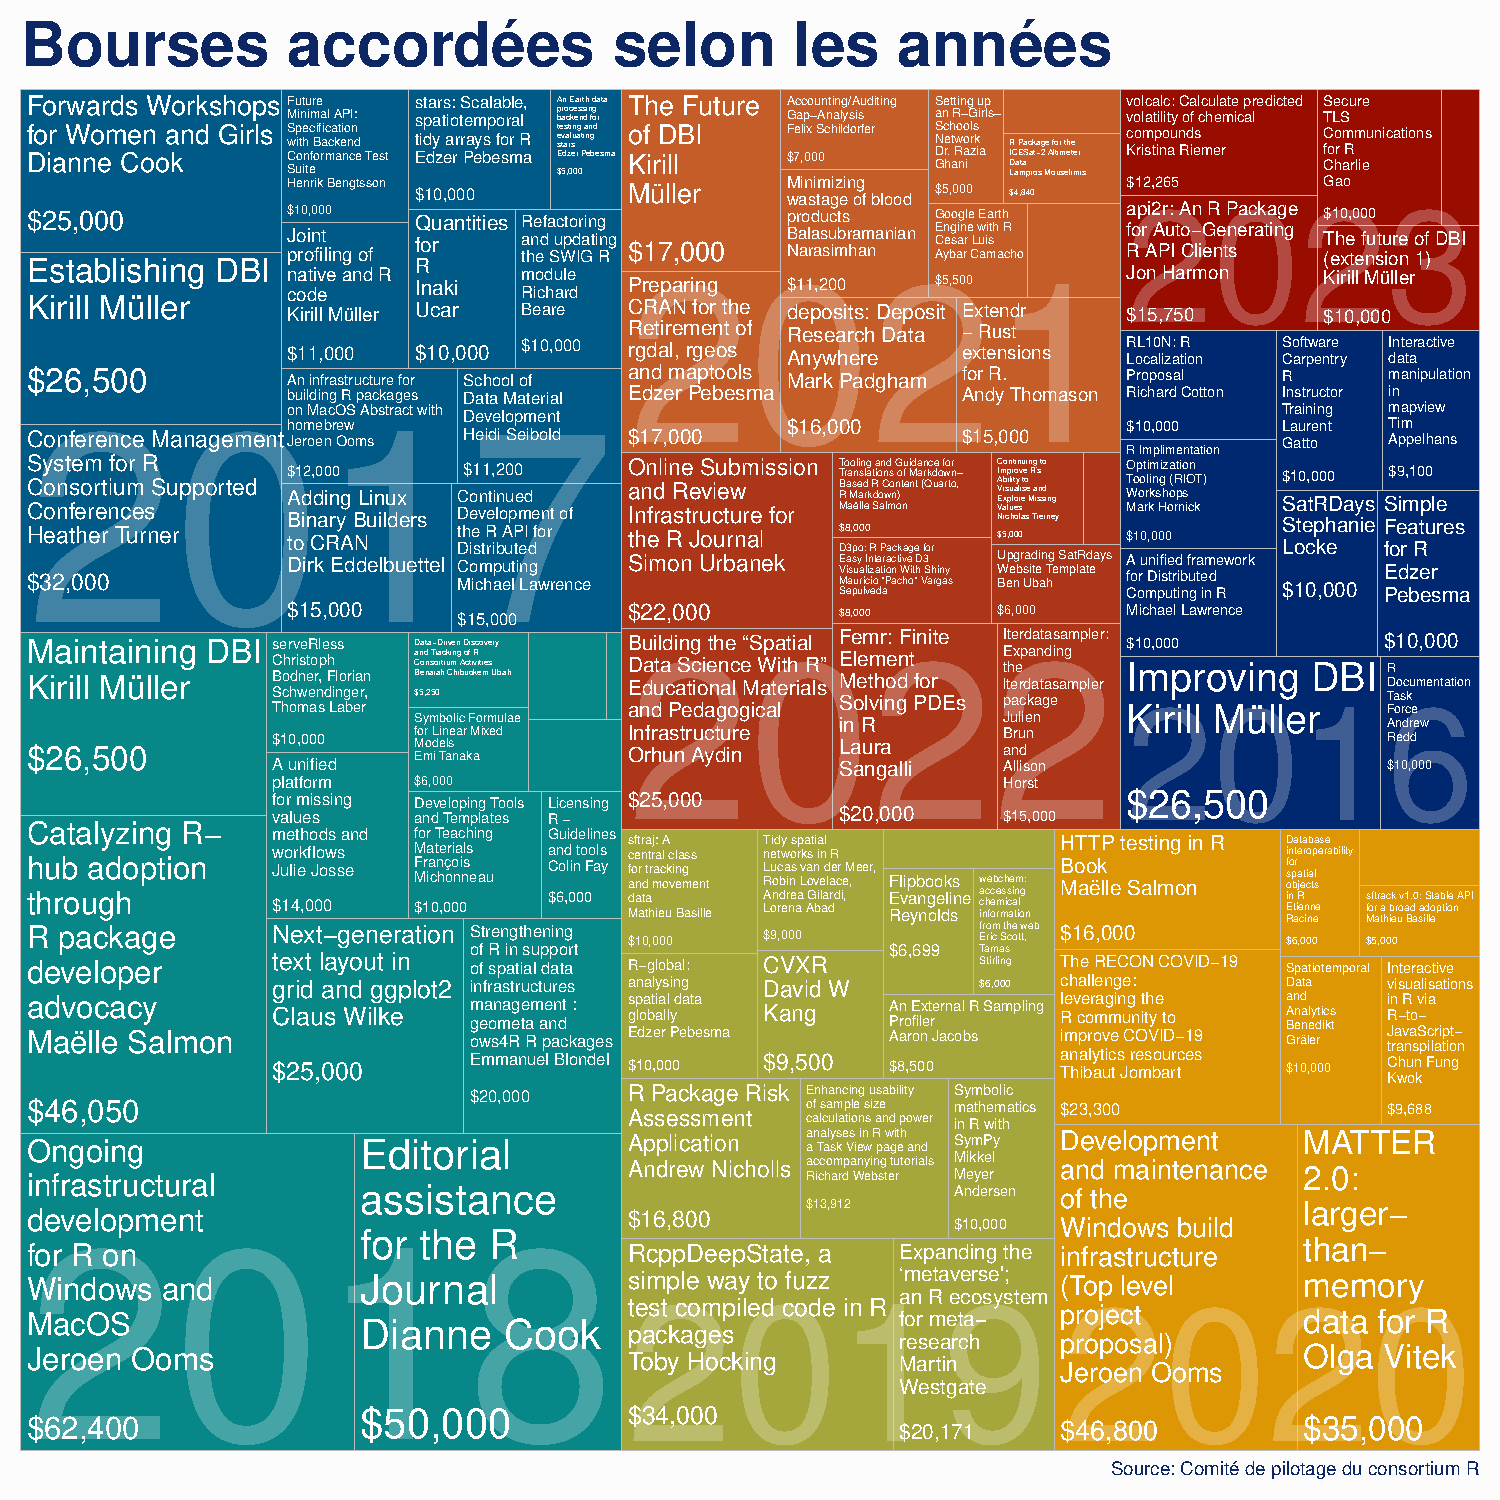
\includegraphics{pw1_VID_files/figure-pdf/unnamed-chunk-28-1.pdf}

}

\end{figure}

Conclusion

En conclusion, cette expérience m'a permis de mettre en pratique
plusieurs aspects fondamentaux de l'analyse de données et de la
visualisation. À travers la manipulation des jeux de données, j'ai pu
développer mes compétences avec les outils tels que R et ses
bibliothèques.

J'ai pu apprendre à créer des visualisations intéressantes, ce projet
m'a permis d'acquérir des connaiisances de base dans la manipulation des
données avec R dans le domaine de la science des données.

J'ai rencontré plusieurs problèmes avec le logiciel Rstudio qui ont
souvent été résolus en redémarrant celui-ci. De plus ne nombreux
problèmes avec certains packages en rapport avec des versions lors
d'appel de fonctions sans vraiment comprendre d'où venait le problème..

Ce cours m'a permis de prendre conscience de l'importance de la
présentation des données et de la clarté dans la communication des
résultats, des compétences indispensables dans ma future carrière en
science des données.



\end{document}
